\documentclass[a4paper]{report}

\usepackage{amssymb}
\usepackage{theorem}
\usepackage[pdftex]{graphicx}
\usepackage{epstopdf}
\usepackage{amsmath} % Include the ast symbol
\usepackage{comment}  % Include the comment function
\usepackage[swedish, english]{babel}
\usepackage{tikz}
\usetikzlibrary{shapes,arrows}
\newtheorem{thm}{Theorem}
\usepackage[T1]{fontenc}
\usepackage{lmodern}
\usepackage[utf8]{inputenc} 
\usepackage{multicol}
\usepackage{graphicx}
\usepackage{subfigure}
\usepackage{tabularx}
\usepackage{multirow}
\usepackage{array}
\usepackage{placeins}



\begin{document}

%%%%%%%%%%%%%%%%%%%%  macro %%%%%%%%%%%%%%%%%%%%%
\def\hath{\hat{H}}
\def\wf {\Psi(\{\bf{R}_\textit{I}, \bf{r}_\textit{i} \})}
\def\wfbo{\Psi_{\textit{bo}}({\textbf{r}_{\textit{i}}},\bf{R} )}
\def\wfh{\Psi_{\textit{h}}(\{\textbf{r}_{\textit{i}}\})}
\def\wfhit<#1>{\Psi_{\textit{h}}^{#1}({\textbf{r}_{\textit{i}}})}
\def\bwf<#1><#2>{\phi_{#1}(\textbf{r}_{#2})}
\def\bwfn<#1><#2>{\phi_{#1}(\textbf{r}{#2})}
\def\wfbloch<#1><#2>{\Psi_{#1,#2}(\textbf{r})}
\def\ubloch<#1><#2>{u_{#1,#2}(\textbf{r})}
\def\ebloch<#1><#2>{E_{#1,#2}}
\def\bwfc<#1><#2><#3>{\phi_{#1}^{#3}(\textbf{r}_{#2})}
\def\sumi<#1> {\sum\limits_\textit{#1}}
\def\sumij<#1><#2> {\sum\limits_\textit{#1,#2}}
\def\suminj<#1><#2> {\sum\limits_{\textit{#1} \neq \textit{#2}}}
\def\coefkhe{-\frac{\hbar^2}{2 m_\textit{e}}}
\def\coefkhn{-\frac{\hbar^2}{2 M_\textit{I}}}
\def\nablai2<#1> {{\nabla}_{\textit{#1}}^{2}}
\def\moperater{-i\hbar \nabla}
\def\sumg<#1>{{\sum\limits_{\bf{#1}}}}    
\def\sumlm<#1><#2>{\sum\limits_{{#1}{#2}}}
\def\coeff<#1><#2><#3>{C_{#1,\bf{k_0}+\bf{#2}}^{#3}}      %C_{j,k_0+G}^{*}
\def\expkg<#1><#2>{e^{i(\bf{#1}+\bf{#2})\bf{r}}}          %exp{i(k+G)r}
\def\expg<#1>{e^{i\bf{#1}\bf{r}}}                         %exp{iGr}
%\def\bwf<#1>{\phi_{\bf{k_0}+\bf{#1}}^{\textbf{APW}}(\textbf{r})}          %phi_{k_0+G}  
\def\chig<#1>{{\chi_{\bf{kk_0}}(\bf{#1})}}                  %chi_{kk_0}{G}
%\def\hath{ | \hat{H} | }           
\def\kplusg<#1><#2>{(\bf{#1}+\bf{#2})}                    % k+G 
\def\radiaf<#1><#2>{f_{{\ell}^{\prime}{m}^{\prime}} (r_{\alpha},\bf{#1+#2})}    % f(r,k+G)
\def\radiafc<#1><#2><#3>{f_{{\ell}^{\prime}{m}^{\prime}}^{#3} (r_{\alpha},\bf{#1+#2})}    % f(r,k+G)
\def\bradiaf{u^{\alpha}_{q,\ell^{\prime}}(r_{\alpha},E_{\ell^{\prime}})}              %u(r_\alpha) did not contain the Energy
\def\sphfr<#1><#2><#3> {{Y_{#1}^{#3}(\hat{\bf{#2}}_{\alpha})}}                             %Y_{lm}(\hat{r})
\def\sphfq<#1><#2><#3> {{Y_{#1}^{#3}(\hat{\bf{#2}})}}                             %Y_{lm}(\hat{q})
\def\gaucoe{C_{{\ell{m}},{\ell^{\prime}m^{\prime}},{\ell^{\prime\prime}m^{\prime\prime}}}}  %Gaunt coefficient
\def\potvgir{V_{\bf{G^{\prime\prime}}}}                                %V{G}
\def\potvmt{V^{\alpha}_{{\ell}^{\prime\prime}{m}^{\prime\prime}} (r_{\alpha})}  %V{lm,r}   
\def\fracatom<#1> {e^{i\bf{#1}\bf{R^\alpha}}}   % exp(iqR)
\def\bessf<#1>{j_{\ell}({#1}r_{\alpha})}     %j_l(kr)
\def\dr{\mathrm{d}\bf{r}}
\def\chikp<#1><#2>{{\chi_{#1,#2}(\textbf{r})}}  
\newcommand{\se}{Schrödinger equation}
\def\hm{Hamiltonian }
\def\cigs{CuIn_{1-\textit{x}}Ga_{x}Se_2}
\def\czts{Cu_2ZnSnS_2}
\def\cztse{Cu_2ZnSnSe_2}
 

\title{Licenciate}
\author{Rongzhen Chen}
\date{?????}

\maketitle

\pagenumbering{roman}
%\tableofcontents
%\listoffigures
%\listoftables



\pagenumbering{arabic}

\begin{abstract}
\noindent In order to reduce the high dependence on fossil fuels and oil, solar energy is one of the alternatives.
There are several very important absorber materials in the thin film photovlotaic technology, such as, the chalcopyrite $\cigs$ (CIGS), $\czts$ (CZTS) and $\cztse$ (CZTSe),
the efficiency of CIGS has been reached up to around 20\%, so the accurate information for this kind of absorber materials is of great importance in order to
design the photovlotaic materials. 

\noindent In this licenciate, the parameterization of the band dispersion for the uppermost three valence bands (VBs) and the lowest conduction
band (CB) in CIGS with $x=0, 0.5$, and $1$ is explored, which is based on the $k \cdot p$ method, but extended it up to high order. It demonstates that the VBs and CB
are quite non-parabolic away from the $\Gamma$ point, which means that the effecive mass on $\Gamma$ point is not suitable to discribe the materials preperties like 
band filling and strong excitation effects. At last, the $\varepsilon = [2\varepsilon_{\perp}+\varepsilon_{\parallel}]/3$ spectra of $CuIn_{0.5}Ga_{0.5}Se_2$ is calculated, and compared with the
experiment result from $CuIn_{0.7}Ga_{0.3}Se_2$ at 40 K, which demonstates that the overall shape of $\varepsilon$ spectra both of calculated and experimented 
is in good agreement.

\noindent The lowest CB and three uppermost VBs of CIGS is parameterized in order to better understand and discribe the anisotropy and non-parabolic of the energy dispersion.
In order to illustrate the non-parabolic of the band dispersion, the effective electron and hole mass tensors are abtained in four symmetry dirctions, to futher illustrate
the non-parabolic, the constant energy surface are calculated for the three topmost VBs as well as the lowest CB. Based on the non-parablic parameterization and compared
with parabolic band energy module, the density-of-states (DOS), the carrier concentrations and Fermi energy are calculated and analyzed. Thus, 


\noindent The $\varepsilon$ spectra of $CuIn_{0.5}Ga_{0.5}Se_2$ is determined by the full-potential linearized augmented plane wave calculations (FPLAPW), which shows a good 
agreement with the result from Spectroscopic ellipsometry, which illustrates the result of $CuIn_{0.7}Ga_{0.3}Se_2$ at 40 K, furthermore, the probable electronic origins of 
observed interband critical points (CP) is discussed, and the electronic orgins of each CP are examined based on the calculation results from the FPLAPW calculations, at 
last, the band to band analysis of the contribution to the total ${\varepsilon_2}$ spectrum is explored.

\end{abstract}


\chapter{Introduction }









\chapter{Electronic structure calculations }
\label{ch:dft}

\section{The quantum many-body problem}
\label{ch:mb}

\noindent The solid is a set which includes a huge amount of atoms (around $10^{23}/cm^3$), and the atom is constructed by nuclei and electrons. 
According to the quantum mechanics principles, we will know all the properties of solid matter if we can figure out a way to solve 
the quantum many-body Schrödinger equation exactly. Let us start from the time-independent many-body Schrödinger equation,

 
\begin{equation}\label{ssth}
 {\hath} {\wf} = {E} {\wf}
\end{equation}

\noindent where $\wf$  is the exact wavefunction for the above Schrödinger equation, $\textbf{r}_\textit{i}$ and $\textbf{R}_\textit{I}$  stands for electron and nucleus coordinators,
respectively, $E$ is the energy of the system, $\hath$ is Hamiltonian which has the following form:

\begin{equation}\label{th}\begin{split}
&\hath = - \sumi<i> {\frac{\hbar^{2}}{2 m_\textit{e}}}   \nablai2<i> - \sumi<I> {\frac{\hbar^{2}}{2 M_\textit{I}}} \nablai2<I>  - \sumij<i><I> \frac{Z_\textit{I}\ e^2}{4 \pi \varepsilon_0 |\textbf{r}_\textit{i}-\textbf{R}_\textit{I}|} \\
& + \frac{1}{2} \suminj<i><j> \frac{ e^2}{4 \pi \varepsilon_0 |\textbf{r}_\textit{i}-\textbf{r}_\textit{j}|} + \frac{1}{2} \suminj<I><J> \frac{Z_\textit{I} Z_\textit{J}\  e^2}{4 \pi \varepsilon_0 |\textbf{R}_\textit{I}-\textbf{R}_\textit{J}|}
\end{split}\end{equation}


\noindent where the indices $\textit{i}$, $\textit{j}$ are used for electron and $\textit{I}$, $\textit{J}$ are used for atomic nuclei, $Z_\textit{I}$ means the charge of the $\textit{I}$-th nucleus,
here  $\textit{I}$ is a number, and ($\textit{I}$)-th means the ordinal number of $\textit{I}$, $\textit{M}$ denotes nuclear mass, $m_e$ is the electron mass, $\varepsilon_0$ is vacuum permittivity.

\noindent The equation \ref{th} has the following form in atomic units:
\
\begin{equation}\label{sth}\begin{split}
&\hath = - \sumi<i>   \frac{{{\nabla}_{\textit{i}}^{2}}}{2} - \sumi<I> \frac{{{\nabla}_{\textit{I}}^{2}}}{2 M_\textit{I}}  - \sumij<i><I> \frac{Z_\textit{I}}{|\textbf{r}_\textit{i}-\textbf{R}_\textit{I}|} \\
& + \frac{1}{2} \suminj<i><j> \frac{1}{ |\textbf{r}_\textit{i}-\textbf{r}_\textit{j}|} + \frac{1}{2} \suminj<I><J> \frac{Z_\textit{I} Z_\textit{J}\ }{|\textbf{R}_\textit{I}-\textbf{R}_\textit{J}|}
\end{split}\end{equation}


\noindent In equation \ref{sth}, the first and second terms are the kinetic energy operator of the electron and nuclei, respectively,
and the other terms in order are Coulomb interaction between electrons and nuclei, electrons and electrons and nuclei and nuclei.

\noindent Since there are so many atoms to calculate in reality, more importantly, we don't know exactly the form of the wavefunction neither,
so we can not solve the equation \ref{ssth} exactly at present, but people already figure out some ways to approximate the exact solution. 
Generally we can divide these approximations into three different levels, the first level is the Born-Oppenheimer approximation and the second level is Hartree,
Hartree-Fock (HF), density functional theory (DFT) and kohn-sham (KS) equation, the last level is the approximation for solving the secular equation, which is an equation that is solved to find the eigenvalue of matrix.

\section{The Born-Oppenheimer approximation}
\label{ch:boa}
\noindent In order to simplify the equation  \ref{ssth}, the first attempt is to seperate the wavefunction of electrons and nuclei, i.e., 
$\wf = {\theta(\bf{R})} {\Psi(\bf{r})} $, but since there is a couple term between the electron and nucleus in the Schrödinger Hamitonian in equation \ref{sth}, 
so we can not do that simply. On the other hand, let us look at the equation
\ref{sth} again, and we can find that there is a “small” value ${1}/{M}$, which is part of the nucleus kinetic energy
operator term, the reason is that the mass of nucleus is much larger than that of electron, so if we treat the mass
as infinity, the result is that the electron is seen as interacting under both the “external” potential caused by nuclei that are fixed in 
some positions and that of other electrons. We can see more vividly description from Figure 1 below.
%figure
\begin{figure}[!htb]
\centering
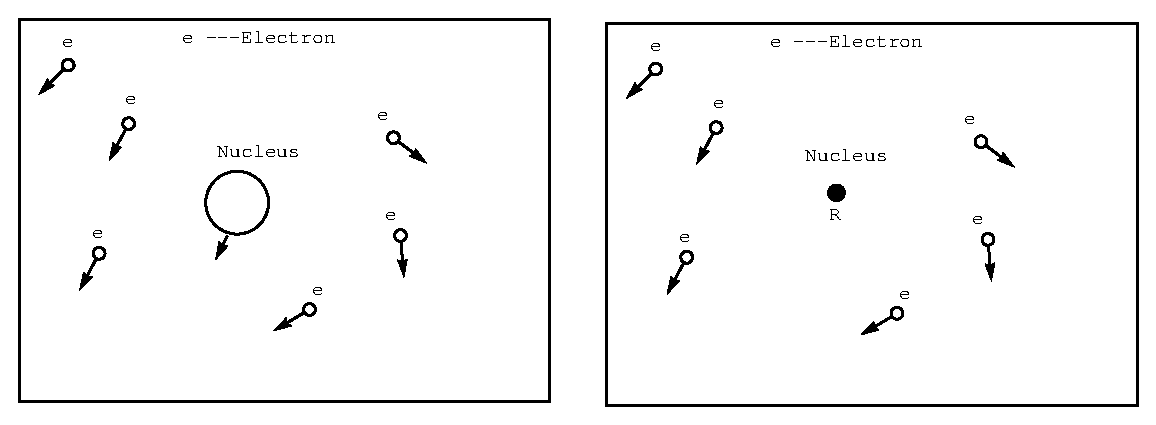
\includegraphics[scale=.5]{system.eps}
\caption{Left one: normal interacting system. Right one. The born-Oppenheimer approximation. The arrow denotes the movement of the nucleus or electron}
\label{fig:bo}
\end{figure}

\noindent The separation of motion between electrons and nuclei is called the Born-Oppenheimer approximation, since the position of nuclei is fixed, so we can define

\begin{equation}\label{nwf}
{\wf}  {\approx}  {\Psi_{ \textit{bo}} ( \{ {\textbf{r}_{\textit{i}}},\bf{R} \}) } = {\theta(\bf{R})} {\Psi(\bf{r}, \bf{R})}
\end{equation}

 \noindent where $\Psi_{ \textit{bo}} ( \{ {\textbf{r}_{\textit{i}}},\bf{R} \})$  is the wavefunction of electrons for Born-Oppenheimer approximation, $\bf R$ is only discrete value belonging to the set of atomic positions, 
 so now, we can recheck the equation \ref{sth} again, we find out that the term of nuclei kinetic is gone, the term of interacting
 between nuclei is simplified as a constant. Now, we can redefine the equation \ref{sth} as follows:

\begin{equation}\label{both}\begin{split}
&{\hath}_\textit{bo}\ =\ - \sumi<i>   \frac{{{\nabla}_{\textit{i}}^{2}}}{2}  - \sumi<i> V_{ext}(\textbf{r}_{\textit{i}})  + \frac{1}{2} \suminj<i><j> \frac{1}{ |\textbf{r}_\textit{i}-\textbf{r}_\textit{j}|} + \frac{1}{2} \suminj<I><J> \frac{Z_\textit{I} Z_\textit{J}\ }{|\textbf{R}_\textit{I}-\textbf{R}_\textit{J}|} \\
&\ = \ \hat{T} \ + \ \hat{V}_\textit{ext} \ + \ \hat{V}_\textit{int}\ + \ N_\textit{II}
\end{split}\end{equation}

\noindent where ${\hath}_\textit{bo}$  is the Hamitonian corresponding the Born-Oppenheimer approximation, the second term is the nuclei potential acting on the
electrons, 

\begin{equation}
V_{ext}(\textbf{r}_{\textit{i}}) =  \sumi<I> \frac{Z_\textit{I}}{|\textbf{r}_\textit{i}-\textbf{R}_\textit{I}|}
\end{equation}

\noindent where the subscript “$ext$” in the second term means “$external$”, so this term is about external potentials interaction. 
The corresponding Schrödinger equation is:

\begin{equation}\label{bose}
{\hath}_{bo} \wfbo = E_\textit{bo} {\wfbo}
\end{equation}

\noindent where $E_\textit{bo}$ is the energy of this electronic system. So far,
the discussion above is only considering the Schrödinger equation of electron, i.e., equation \ref{bose}, so how about the Schrödinger equation of nucleus? First, comparing equation
\ref{sth} and \ref{both}, we can rewrite the total Schrödinger Hamitonian as 

\begin{equation}\label{nh}
 {\hath} = - \sumi<I> \frac{{{\nabla}_{\textit{I}}^{2}}}{2 M_\textit{I}} + {\hath}_{bo}
\end{equation}

\noindent so the new Schrödinger equation with equation \ref{nh} and \ref{nwf} is 

\begin{equation}
 (- \sumi<I> \frac{{{\nabla}_{\textit{I}}^{2}}}{2 M_\textit{I}} + {\hath}_{bo} ) ( {\theta(\bf{R})} {\Psi(\bf{r}, \bf{R})}) = E_{m}({\bf R}) ({\theta(\bf{R})} {\Psi(\bf{r}, \bf{R})} )
\end{equation}
 
\noindent where $E_{m}$ is the total energy of above system, after some steps of derivation, we can end up with the following equation:
\begin{equation}\label{ise}
( \hat{H}_{I1}+\hat{H}_{I2}+\hat{H}_{I3}+E_{bo}({\bf R}) ) {\theta(\bf{R})} = {E_m} {\theta(\bf{R})}
\end{equation}

\noindent where

\begin{equation}\begin{split}
 &  \hat{H}_{I1} = - \sumi<I> \frac{{{\nabla}_{\textit{I}}^{2}}}{2 M_\textit{I}}   \\
 &  \hat{H}_{I2} = - \sumi<I> \frac{1}{M_\textit{I}} {\int {\Psi(\bf{r}, \bf{R})}^{\ast} {{\nabla}_{\textit{I}}} {\Psi(\bf{r}, \bf{R})} d {\bf r }} {{\nabla}_{\textit{I}}} \\
 &  \hat{H}_{I3} = - \sumi<I> \frac{1}{M_\textit{I}} {\int {\Psi(\bf{r}, \bf{R})}^{\ast} {{\nabla}_{\textit{I}}^{2}} {\Psi(\bf{r}, \bf{R})} d {\bf r }} 
\end{split}\end{equation}

\noindent from equation \ref{ise}, we obsever that we can get the lattice dynamical properties of certain system within the Born-Oppenheimer approximation, and in this equation,
we also need the gournd state energy $E_{bo}({\bf R})$ of electron system to solve equation \ref{ise}, here $\bf R$ is the parametrilized value from the atom position.
 

\noindent In summary, we derive the Schrödinger equation of electron and nucleus seperatly in this section, and usually, when we refer to calculate the ground state properties,
we means to take use of the Schrödinger equation of electron only, e.g., equation \ref{bose}, and we use Schrödinger equation of nucleus for the calculation of lattice dynamics.

So far, we notice that the equation \ref{both} is much simpler than equation \ref{sth}, but still not solvable, so we need further more excellent approximations 
to solve this many-body problem.


\section{Hartree and Hartree-Fock approximation}
\noindent Hartree or Hartree-Fock method is straightforward to get the 
expression we are expecting using the mathematical approaches, and both of them focus on the treatment of wavefunction, however, the wavefunction in Hartree method is not 
flexible enough, and better but not enough (lacking of correlation term) in Hartree Fock method.

%the density functional theory (DFT) is a perfect method which can solve the 
%many-body equation in theory, but not solvable in practice

\subsection{Hartree approximation}
\label{ha}
\noindent The simplest approximation of the wavefunction for many-body Schrödinger equation is the form of acting like non-interacting 
electrons, so the wavefunction with N non-interacting electrons has the following expression:

\begin{equation}\label{wfh}
\wfh = \bwf<1><1> \bwf<2><2> \cdots \bwf<N><N> 
\end{equation}

\begin{comment}
\begin{equation}\label{wfh}
\langle \rangle
\end{equation}
\end{comment}


\noindent where $i$ goes through all the electrons, and  means state of the $i$-th electron in the position of ${\textbf{r}}_{\textit{i}}$, 
from here and following the $R$ is suppressed in the wavefunction since they are position fixed. So the total energy of the system we can write down in the following way :

\begin{equation}\label{teh}
E_{\textit{h}} = <\wfh |\ {\hath}_{\textit{bo}} \ | \wfh  >
\end{equation}

\noindent So making the substitution using equation \ref{both} and \ref{wfh} into equation \ref{teh}, we can get the total energy of system:
\begin{equation}\begin{split}
&E_\textit{h} = \sumi<i> <\bwf<i><> |\ -\frac{\nabla^{2}_{\textit r}}{2} + V_\textit{ext}(\textbf{r})  \ | \bwf<i><> > \\
& +\frac{1}{2} \suminj<i><j> <\bwf<i><> \bwfn<j><'>|\ \frac{1}{|\textbf{r} - \textbf{r}^{'} |} \ | \bwf<i><> \bwfn<j><'>>
\end{split}\end{equation}

\noindent In order to calculate the stationary state of the system, so the variation of the wavefunction should be
zero variation in the energy, so here we can set up the following equation with Lagrange multiplier $E^{i}_h$
\begin{equation}\label{haa}
 \delta [ E_{\textit{h}} - \sumi<i> E^{i}_{h} (<\bwf<i><> | \bwf<i><> > -1)] = 0 
\end{equation}

\noindent In order to calculate the term $\delta ( E_{\textit{h}} ) $, we have to know
\begin{equation}\begin{split}\label{hartree1}
& \delta ( \sumi<i> <\bwf<i><> |\ -\frac{\nabla^{2}_{\textbf r}}{2} + V_\textit{ext}(\textbf{r})  \ | \bwf<i><> > ) \\
&  = \sumi<i> \{ < \delta \bwf<i><> |\ -\frac{\nabla^{2}_{\textbf r}}{2} + V_\textit{ext}(\textbf{r})  \ | \bwf<i><> >  
   + <  \delta \bwf<i><> |\ -\frac{\nabla^{2}_{\textbf r}}{2} + V_\textit{ext}(\textbf{r})  \ |  \bwf<i><> >^{\ast} \}
\end{split}\end{equation}

\noindent and 

\begin{equation}\begin{split}\label{hartree2}
&  \delta( \frac{1}{2} \suminj<i><j> <\bwf<i><> \bwfn<j><'>|\ \frac{1}{|\textbf{r} - \textbf{r}^{'} |} \ | \bwf<i><> \bwfn<j><'>>)   \\
& =   \frac{1}{2} \suminj<i><j> \{  <\delta \bwf<i><> \bwfn<j><'>|\ \frac{1}{|\textbf{r} - \textbf{r}^{'} |} \ | \bwf<i><> \bwfn<j><'>>  \\
& +   < \bwf<i><> \delta \bwfn<j><'>|\ \frac{1}{|\textbf{r} - \textbf{r}^{'} |} \ | \bwf<i><> \bwfn<j><'>> +  T_{rem}\}
\end{split}\end{equation}

\noindent where $T_{rem}$ is the remaining terms, actually these remaining terms will not affect the derivation. Before getting the final result, 
there is one more identity 

\begin{equation}\begin{split}\label{hartreelabel1}
& < \bwf<i><> \delta \bwfn<j><'>|\ \frac{1}{|\textbf{r} - \textbf{r}^{'} |} \ | \bwf<i><> \bwfn<j><'>> \\
& = \int d \textbf{r} d \textbf{r}{'}  \phi_{i}^{*} (\textbf{r}{}) \delta \phi_{j}^{*} (\textbf{r}{'}) \frac{1}{|\textbf{r} - \textbf{r}^{'} |}  \phi_{i}^{} (\textbf{r}{})  \phi_{j}^{} (\textbf{r}{'})\\
& = \int d \textbf{r}{'} d \textbf{r}  \phi_{i}^{*} (\textbf{r}{'}) \delta \phi_{j}^{*} (\textbf{r}{}) \frac{1}{|\textbf{r}{'} - \textbf{r} |}  \phi_{i}^{} (\textbf{r}{'})  \phi_{j}^{} (\textbf{r})\\
& = <\delta \bwf<j><> \bwfn<i><'>|\ \frac{1}{|\textbf{r} - \textbf{r}^{'} |} \ | \bwf<j><> \bwfn<i><'>>
\end{split}\end{equation}

\noindent So the equation \ref{hartree2} will become 

\begin{equation}\begin{split}\label{hartree3}
&  \delta( \frac{1}{2} \suminj<i><j> <\bwf<i><> \bwfn<j><'>|\ \frac{1}{|\textbf{r} - \textbf{r}^{'} |} \ | \bwf<i><> \bwfn<j><'>>)   \\
& =  \suminj<i><j> \{  <\delta \bwf<i><> \bwfn<j><'>|\ \frac{1}{|\textbf{r} - \textbf{r}^{'} |} \ | \bwf<i><> \bwfn<j><'>> + \frac{T_{rem}}{2}\}
\end{split}\end{equation}


Taking use of the above two equation \ref{haa}, \ref{hartree1}, \ref{hartree3} and variation in the term of  $\delta \phi^{*}_{i}(\textbf{r}{}) $,
finally we end up with
\begin{equation}\label{hha}
(-\frac{\nabla^{2}_{\textbf r}}{2} + V_\textit{ext}(\textbf{r})+ \suminj<j><i> <\bwfn<j><'>\ | \frac{1}{|\textbf{r} - \textbf{r}^{'} |} \ | \bwfn<j><'>>) \bwf<i><> = E^{i}_{h} \bwf<i><>
\end{equation}
\noindent where $E^{i}_{h}$  also can be treated as the energy corresponding the ($i$)-th electron in the position of  $\textbf{r}$, the equation \ref{hha} is a group of dependent single
 particle equations, and after checking it, we can find out which is an equation that is self-consistent and can be solved using
 computer by iteratively.


%%%%%%%%%%%%%%%%%%%%figure
\begin{comment}
\noindent where $\wfhit<0>$ is the initial wavefunction,$\wfhit<m+1>$ and $\wfhit<m>$ are the wavefunction of ($m$)-th the ($m+1$)-th iteration solving the Hartree equation,
 respectively, and $\delta$ is the tolerance.
\end{comment}

\subsection{Hartree-Fock approximation}
\noindent Hartree approximation is the lowest level approximation, and Hartree-Fock approximation is the method which considers the 
antisymmetry of the wavefunction, which means that if the positions of two electrons (with same spin) are exchanged, the wave 
function should change the sign, like:
\begin{equation}\label{hfwf}
\Psi_\textit{hf} (\{ \cdots \textbf{r}_\textit{i} \cdots  \textbf{r}_\textit{j} \}) = - \Psi_\textit{hf} (\{ \cdots \textbf{r}_\textit{j} \cdots  \textbf{r}_\textit{i} \})
\end{equation}
\noindent Slater introduced  an excellent way to construct the wavefunction due to the equation \ref{hfwf} based on the Hartree approximation, 
the wavefunction of many- body Schrödinger equation is written down  in a matrix determinant way for the number of $N$ electrons 
(without spin):
\begin{equation}\label{hfwfm}
\Psi_{hf}(\mathbf{r}_1, \mathbf{r}_2, \ldots, \mathbf{r}_N) =
\frac{1}{\sqrt{N!}} \left|
\begin{matrix}
    \bwf<1><1> & \bwf<1><2> & \cdots & \bwf<1><N> \\
    \bwf<2><1> & \bwf<1><2> & \cdots & \bwf<1><N> \\
    \vdots               & \vdots               &        & \vdots               \\
    \bwf<N><1> & \bwf<N><2> & \cdots & \bwf<N><N>
\end{matrix} \right|
\end{equation}
\noindent where $i$ goes through all the electron, and $\bwf<i><i>$ means state of the ($i$)-th electron in the position of $\textbf{r}_\textit{i}$, so if we exchange two rows
 in the equation \ref{hfwfm}, we will find out the result is satisfied with the equation \ref{hfwf}.

\noindent Now repeating all the processes already done through the Hartree approximation , we will know the total energy of Hartree-Fock as follows:

\begin{equation}\begin{split}
&E_\textit{hf} = \sumi<i> <\bwf<i><> |\ -\frac{\nabla^{2}_{\textit r}}{2} + V_\textit{ext}(\textbf{r})  \ | \bwf<i><> > \\
& + \frac{1}{2} \suminj<i><j> <\bwf<i><> \bwfn<j><'>|\ \frac{1}{|\textbf{r} - \textbf{r}^{'} |} \ | \bwf<i><> \bwfn<j><'>> \\
& - \frac{1}{2} \suminj<i><j> <\bwfn<i><'> \bwfn<j><>|\ \frac{1}{|\textbf{r} - \textbf{r}^{'} |} \ | \bwfn<i><> \bwfn<j><'>>
\end{split}\end{equation}

\noindent In the same mathematical skill but more complicated like in previous section, we can get the dependent singe particle Hartree-Fock equation:

\begin{equation}\begin{split}
& \{ -\frac{\nabla^{2}_{\textit i}}{2} + V_\textit{ext}(\textbf{r})+ \suminj<j><i> <\bwfn<j><'>\ | \frac{1}{|\textbf{r} - \textbf{r}^{'} |} \ | \bwfn<j><'>> \} \bwf<i><>  \\
& - \suminj<i><j>  < \bwfn<j><'>|\ \frac{1}{|\textbf{r} - \textbf{r}^{'} |} \ | \bwfn<i><'> >) \bwfn<j><>  = E^{i}_{hf} \bwf<i><>
\end{split}\end{equation}

\noindent Comparing with Hartree equation, there is an extra term in the equation above, which is called exchange term, and at the same time,
 in order to organize the equation in a nice and clear way, finally we define:
\begin{equation}\begin{split}
\{ -\frac{\nabla^{2}_{\textit i}}{2} + V_\textit{ext}(\textbf{r}) +V_\textit{H}(\textbf{r}) \}  \bwf<i><>  = E^{i}_{hf}   \bwf<i><> 
\end{split}\end{equation}
where
\begin{equation}
 V_\textit{H}(\textbf{r})= \int \frac{\rho(\textbf{r}{'}) - \rho_{\textit{i}}^{\textit{HF}}(\textbf{r},\textbf{r}{'})}{|\textbf{r} - \textbf{r}^{'} |}  \mathrm{d}\textbf{r}^{'}
\end{equation}
and $ \rho_{\textit{i}}^{\textit{HF}}(\textbf{r},\textbf{r}{'}) = \sumi<j> \frac{\phi_{i}^{}(\textbf{r}{'}) \phi_{i}^{*}(\textbf{r}{}) \phi_{j}^{}(\textbf{r}{}) \phi_{j}^{*}(\textbf{r}{'})} {\phi_{i}^{}(\textbf{r}) \phi_{i}^{*}(\textbf{r})} $ 
; $\rho(\textbf{r}) = \sumi<i>  {|\bwf<i><>|}^{2}$ . And also we find that we can solve it in the same way like Hartree approximation but plus one
extra term.

\section{Density functional theory}
\noindent Hartree and Hartree-Fock methods are very classic methods to solve many-body Schrödinger equation. However, HF method only includes the exchange,
 but badly in the electron correlation, so they are not suitable in the case of electrons in solid. Apart from the two methods mentioned before, there is another modern method to deal with
 the more complicated calculation of electrons, namely, density functional theory (DFT), which is introduced by Hohenberg and
 Kohn in 1964, Kohn and Pople was awarded by Chemistry Nobel Prize in 1998.

\noindent The idea of this method is to treat the electron density of solid instead of using the many-particle wavefunction, so we can
 benefit that the degree of freedom reduces from 3N (N is the number of electrons) to 3, which is apparently less complicate than 
those of Hartree and Hartree-Fock during calculation. 

\subsection{The Density as Basic Variable}
\noindent There are two questions coming out if we consider the electron density as the role of wavefunction. The first one is whether it
 is the equivalence relation between the electron density and wavefunction of the system, and the second one is how to solve this 
problem. In order to know that there are two very basic theorems introduced by Hohenberg and Kohn:

\begin{thm}
\label{hk1}
\noindent The first theorem says that the external potential $V_\textit{ext}(\textbf{r})$  is determined uniquely for any of electon system by the ground state electron density $\rho_0$.
\end{thm}

\noindent The above theorem also indicate that all the ground state properties are decied by the true ground state density $\rho_0$,
for example, the total energy E=E[$\rho_0$]. 
\noindent The above theorem also explains the equivalence relation between the electron density and wavefunction, because Hamiltonian is obtained from external potentials,
then one can get the wavefunction, so the corresponding electron density is determined, however, from the theorem, the external potential is unique decided by electron
density, so the electron density contains the same information of wavefunction.

\noindent The proof of theorem is following:

\noindent Now, let us assume that there exsits two external potentials named $V^{1}_\textit{ext}(\textbf{r})$ and $V^{2}_\textit{ext}(\textbf{r})$ leading to the same ground state 
electron density $\rho_0$, but obviously, which will lead to two different Hamiltonians, that is, $\hat{H}_{1}$ and $\hat{H}_{2}$, and as well as two different corresponding
wavefunctions named $\Psi_1$ and $\Psi_2$. Since $\Psi_1$ are not the ground state wavefunction of $\hat{H}_{2}$, the same rules to $\Psi_2$ and $\hat{H}_{1}$, so two following
inequality equations will be satisfied:

\begin{equation}\label{hkpf1}\begin{split}
&  E_1 = \langle \Psi_1\ |\hat{H}_{1}|\ \Psi_1 \rangle  \ < \  \langle \Psi_2\ |\hat{H}_{1}|\ \Psi_2 \rangle\\
&  E_2 = \langle \Psi_2\ |\hat{H}_{2}|\ \Psi_2 \rangle  \ < \  \langle \Psi_1\ |\hat{H}_{2}|\ \Psi_1 \rangle
\end{split}\end{equation}

\noindent Taking advangtage of the form of Hamitonian from equation \ref{both}, one can get:
\begin{equation}\label{hkpf2}\begin{split}
&    \langle \Psi_2\ |\hat{H}_{1}|\ \Psi_2 \rangle \\
&  = \langle \Psi_2\ |\hat{H}_{2} + \hat{H}_{1} - \hat{H}_{2}|\ \Psi_2 \rangle \\
&  = \langle \Psi_2\ |\hat{H}_{2} |\Psi_2 \rangle + \langle \Psi_2 | \hat{H}_{1} - \hat{H}_{2}|\ \Psi_2 \rangle \\
&  = E_2 + \int d \textbf{r} ( V^{1}_\textit{ext}(\textbf{r}) - V^{2}_\textit{ext}(\textbf{r}) )  \rho_0
\end{split}\end{equation}

\noindent So using \ref{hkpf1} and \ref{hkpf2}, one can get:

\begin{equation}\label{hkpf3}
 E_1  < \  E_2 + \int d \textbf{r} ( V^{1}_\textit{ext}(\textbf{r}) - V^{2}_\textit{ext}(\textbf{r}) )  \rho_0
\end{equation}

\noindent Another similar inequality equation will be gained if one changes the form of equation $\langle \Psi_1\ |\hat{H}_{2}|\ \Psi_1 \rangle$ like equation \ref{hkpf2}.
\begin{equation}\label{hkpf4}
  E_2  < \  E_1 + \int d \textbf{r} ( V^{2}_\textit{ext}(\textbf{r}) - V^{1}_\textit{ext}(\textbf{r}) )  \rho_0
\end{equation}

\noindent so plus the left and right sides from equation \ref{hkpf3} and \ref{hkpf4}, one will gain a contradictory result:
\begin{equation}\label{hkpf4}
  E_1 + E_2  < \  E_2 + E_1
\end{equation}

\noindent So the external potential $V_\textit{ext}(\textbf{r})$ is unique.

\begin{thm}
\label{hk2}
\noindent The second theorem says that there is a universal functional for the total energy in the terms of the electron density $\rho$ with any external potential $V_\textit{ext}(\textbf{r})$ ,
and the exact ground state density is gained when the ground state total energy functional reaches its minimal value, that is, E[$\rho$]>E[$\rho_0$], where $\rho$ is not the ground state density.
\end{thm}

\noindent The proof of theorem is following:
Because of the first theorem, so the total energy can be expressed in the following way (ignoring the interaction between nuclei):
\begin{equation}\label{hkpf5}\begin{split}
& E[\rho] \ =\langle \Psi  | \ \hat{T} \ + \ \hat{V}_\textit{int}  \ + \ \hat{V}_\textit{ext} \ | \Psi \rangle \\
&     =\langle \Psi  | \ \hat{T} \ + \ \hat{V}_\textit{int}  \ \ | \Psi \rangle+ \langle \Psi  | \ \hat{V}_\textit{ext} \ | \Psi \rangle \\
&     =\ F[\rho] \ + \ \int \rho(\textbf{r}) V_\textit{ext} 
\end{split}
\end{equation}

\noindent In the above equation \ref{hkpf5}, the term of $F[\rho]$ is the universal functional since all the systems of electrons.

\noindent Now, let us say $\rho_0$ is the exact ground state electron density, from first theorem, we know there exists one unique external potential $V_\textit{ext}$, so 
the corresponding Hamitonian and wavefunction are $\hat{H}$ and $\Psi_0$, assuming that a different electron density $\rho$ which is not exact ground state density 
corresponding to the wavefunction $\Psi_0$, then we will get:

\begin{equation}
E[\rho_0] = \langle \Psi_0\ |\hat{H}|\ \Psi_0 \rangle 
          < \langle \Psi\ |\hat{H}|\ \Psi \rangle \
          = E[\rho]
\end{equation}

\noindent so from above equation, we know the total energy for the case of exact ground state electron density is lower than any other cases, which also means that one can get 
the exact ground state electron density by minimizing the total energy.



\noindent From those two theorems, we definitely know how to solve this problem theoretically, but in practice, we do not know $E[\rho]$, how it looks like, 
so we still need one more method to deal with it, namely, Kohn-Sham (KS) equation.

\section{The Kohn-Sham equation}

\noindent Since I already introduced the Hartree and Hartree Fock method to solve the many-body problem, both of which are based on the idea which is to transform complex 
many-body problem to single particle problem by using wavefunction, but Density functional theory only consider to take use of information from Hamitonian, but not sovable, 
so is it possbile to combine these two ideas together? the answer is yes,the DFT is solved by Kohn-Sham equation introduced by Kohn and Sham in 1965,
which I recommended a way to construct in the following text (ignoring the interaction between nuclei)

\noindent First of all, the total energy can be expressed by the following:
\begin{equation}
\label{kse}
\begin{split}
&E[\rho] \ =\ T[\rho] \ + \ V_\textit{int}[\rho] \ + \ V_\textit{ext}[\rho]  \\
&\ \ \   = \underbrace{\ (T[\rho] \ - \ T_{0}[\rho]) \ + \  (V_\textit{int}[\rho] \ - \ V_\textit{HF}[\rho])\ }+ \ T_{0}[\rho] \ + \ V_\textit{HF}[\rho] \ + V_\textit{ext}[\rho]       \\
&\ \ \   = \ T_{0}[\rho] \ + \ V_\textit{HF}[\rho] \ + \ V_\textit{C}[\rho] +\ V_\textit{ext}[\rho]
\end{split}
\end{equation}
\noindent where $E[\rho]$  is the total energy, $\rho$ is the ground state density;$V_\textit{int}[\rho]$, $T[\rho]$ and $V_\textit{int}[\rho]$ are the energy from external potential, the exact kinetic 
and the exact electron-electron potential energy; $T_{0}[\rho]$ is the kinetic energy of a non-interacting electrons, $V_\textit{HF}[\rho]$ is the potential  from Hartree-Fock approximation.

\noindent From the Hartree-Fock approximation, we can further know that:
\begin{equation}
 V_\textit{HF}[\rho] \ = \ V_\textit{H}[\rho] \ + \ V_\textit{X}[\rho] 
\end{equation}

\noindent where $V_\textit{H}[\rho]$ and $ V_\textit{X}[\rho] $ are the Hartree contribution and exchange contribution, respectively, so the equation (13) can be further defined like
 the following:
\begin{equation}\label{ccc}
\begin{split}
&E[\rho]\ = \ T_{0}[\rho] \ + \ V_\textit{H}[\rho] \ + \ V_\textit{ext}[\rho] \ + \ \underbrace{\ V_\textit{X}[\rho]  \ + \ V_\textit{C}[\rho]}  \\
&\ \ \ = \ T_{0}[\rho] \ + \ V_\textit{H}[\rho] \ + \ V_\textit{ext}[\rho] + \ V_\textit{XC}[\rho]
\end{split}\end{equation}
\noindent where $V_\textit{XC}[\rho]$  is the exchange-correlation term. From equation \ref{kse}, the explicit expression of $V_\textit{XC}[\rho]$ we do not know. 
 but the first three terms we already know

\begin{equation}
 T_{0}[\rho]\ = \ < \Psi_{i}(\textbf{r}) \ | -\frac{\nabla^{2}_{r}}{2} \ | \Psi_{i}(\textbf{r}) >
\end{equation}

\begin{equation}
V_\textit{H}[\rho] \ = \ \frac{1}{2} \int \int \mathrm{d} {\textbf{r}} \mathrm{d}{\textbf{r}^{\prime}} \frac{\rho({\textbf{r}})\rho(\textbf{r}^{\prime})}{|{\textbf{r}}-{\textbf{r}}^{\prime}|} 
\end{equation}


\begin{equation}
V_\textit{ext}[\rho]\ = \ \int \mathrm{d}{\textbf{r}} \rho(\textbf{r}) V_\textit{ext} 
\end{equation}

\noindent In order to derive the ground state of the above system, we can view this problem as the process of minimizing the total energy by varying the wavefunction $\Psi^*$, since
we can construct from wavefunction to electron density (equation \ref{ks1}), just like the derivation in the section of Hartree, we finally can get the Kohn-Sham equation.
\begin{equation}\label{aaa}
 (-\frac{\nabla^{2}_{r}}{2}\ + \ V_\textit{KS}) \Psi_{\textit{i}}(\textbf{r}) = E_{\textit{ks}}^{\textit{i}} \Psi_{\textit{i}}(\textbf{r})
\end{equation}

\noindent where
\begin{equation}\begin{split}
&\ V_\textit{KS} \ = \ V_\textit{ext}[\rho] + \int \frac{\rho(\textbf{r}^{\prime})}{|{\textbf{r}}-{\textbf{r}}^{\prime}|} \ + \ \frac{\delta{E_\textit{XC}}}{\delta{\rho(\textbf{r})}} \\
&\ = \ \ V_\textit{ext}[\rho] + \int \frac{\rho(\textbf{r}^{\prime})}{|{\textbf{r}}-{\textbf{r}}^{\prime}|} \ + \ \upsilon_\textit{xc}
\end{split}
\end{equation}

\noindent we can think of the Hamiltonian in another point of view, e.g., single particle system with three different potentials. Now the
 problem turns out to be like the single particle form with the degree of freedom of 3.

\noindent So the many-body problem now is transformed to the single electron problem, if the $\upsilon_\textit{xc}$  is exact, the exact ground-state density is :
\begin{equation}\label{ks1}
 \rho(\textbf{r}) = \sumi<i> {\Psi^{*}_{i}(\textbf{r})} {\Psi_{i}(\textbf{r})}
\end{equation}

\noindent There is no total energy equation expression yet, however, if one can change the equation \ref{aaa} as 
\begin{equation}\label{bbb}
\sumi<i> \Psi^{*}_{\textit{i}}(\textbf{r})(-\frac{\nabla^{2}_{i}}{2}\ + \ V_\textit{KS}) \Psi_{\textit{i}}(\textbf{r}) = \sumi<i> \Psi^{*}_{\textit{i}}E_{\textit{ks}}^{\textit{i}} \Psi_{\textit{i}}(\textbf{r})
\end{equation}

\noindent Based on equation \ref{ccc} and \ref{bbb}, we will get the total energy expression:
\begin{equation}\label{totalenergy}
\begin{split}
& E= \sumi<i> E_{\textit{ks}}^{\textit{i}} - \ \frac{1}{2} \int \int \mathrm{d} {\textbf{r}} \mathrm{d}{\textbf{r}^{\prime}} \frac{\rho({\textbf{r}})\rho(\textbf{r}^{\prime})}{|{\textbf{r}}-{\textbf{r}}^{\prime}|} \\
&    + \ V_\textit{XC}[\rho] - \int   \upsilon_\textit{xc} \rho({\textbf{r}})
\end{split}
\end{equation}

\noindent So far there are two problems still in the air, one is the exact format of $\upsilon_\textit{xc}$, the other one is how to solve the Kohn-Sham equation.

\section{The exchange-correlation energy}
\noindent This part is the most difficult part during the process of solving the Kohn-Sham equation, because it is unknown so far, so there
 are varies of approximations about it, like the local density approximation (LDA), generalized-gradient approximation (GGA) and
so on.
\subsection{The local density approximation}
\noindent The local density approximation is the simplest way to approximate the exchange-correlation part, and the idea is that the value 
of the exchange-correlation energy in the very tiny small volume is equal to the homogeneous electrons with the same density in 
the volume, the explicit equation is: 
\begin{equation}
 E^\textit{LDA}_\textit{xc} = \int \rho(\textbf{r}) \varepsilon_\textit{xc}( (\rho(\textbf{r})) ) \mathrm{d} \textbf{r} 
\end{equation}

\noindent where $ E^\textit{LDA}_\textit{xc} $ is the exchange-correlation energy functional for the $LDA$, $\rho(\textbf{r})$ is the charge density in the position of $\textbf{r}$, $\varepsilon_\textit{xc}$ is homogeneous 
electrons gas with variable of  $\rho(\textbf{r})$ .

\noindent The $\varepsilon_\textit{xc}$ is an ideal state within a solid, which assumes that the charge is homogeneously all over the space:
\begin{equation}
 \rho(\textbf{r}) = \rho = \frac{N}{V}
\end{equation}

\noindent Where $N$ is number of electrons within the solid, and $V$ is the volume of solid, which also means that the $\varepsilon_\textit{xc}$ is the function of $\rho(\textbf{r})$,
 not functional. 
\subsection{The Generalized gradient approximation}
\noindent The GGA is the approximation beyond the LDA, which incorporates not only the density within the tiny volume, but also the gradient
 of the density, the explicit equation is:

\begin{equation}
E_{\textit{GGA}}^{\textit{xc}}\ = \ \int \rho(\textbf{r}) \varepsilon_\textit{xc}( (\rho(\textbf{r})), \nabla \rho(\textbf{r}) ) \mathrm{d} \textbf{r} 
\end{equation}

\noindent where  is the exchange-correlation energy functional for the GGA,  is the gradient  of charge density in the position of r.

\noindent Of course, there are more modern methods to approximate the exchange-correlation energy, such as: the optimized effective potential
(OEP) method and the hybrid functionals and so on.

\section{Solving the secular equation}
\noindent The process for solving Kohn-Sham equation can be solved by iteration as well, but the difference between for solving Kohn-Sham 
equation and Hartree or Hartree-fock equation is that the wavefunction is replaced by the electron density, so first an initial 
electron density is defined by some way, and later on the equation is solved iteratively until the reasonable solution is obtained.

%%%%%%%%%%%%%%%%%%%%figure
\tikzstyle{decision} = [diamond, draw, fill=white!20,
    text width=10em, text badly centered, node distance=2.5cm, inner sep=0pt]
\tikzstyle{block} = [rectangle, draw, fill=white!20,
    text width=12em, text centered, rounded corners, minimum height=3em]
\tikzstyle{line} = [draw, very thick, color=black!50, -latex']

\begin{figure}[!htb]
\centering


\begin{tikzpicture}[scale=0.6 , node distance = 2.5cm,transform shape]
    % Place nodes
    \node [block] (init) {Initialize/Get density $\rho^{i}$};
    \node [block, below of=init] (potential) {Calculate potential $V( {\bf r})$};
    \node [block, below of=potential, node distance=2.5cm] (KS) {Solve KS equation on each k-point};
    \node [block, below of=KS, node distance=2.5cm] (fermi) {Decide fermi energy $E_F$};
    \node [block, below of=fermi, node distance=2.5cm] (density) {Calculate new density $\rho^{new}$};
    \node [block, left of=fermi, node distance=6cm] (update) {Decide the mix density $\rho^{i+1} = F (\rho^{i}, \rho^{new}) $};
    \node [decision, below of=density, node distance=3.8cm] (converge) {Converged?};
    \node [block, below of=converge, node distance=3.8cm] (done) {Finished};
    % Draw edges
    \path [line] (init) -- (potential);
    \path [line] (potential) -- (KS);
    \path [line] (KS) -- (fermi);
    \path [line] (fermi) -- (density);
    \path [line] (density) -- (converge);
    \path [line] (converge) -| node [near start, color=black] {No} (update);
    \path [line] (update) |- (init);
    \path [line] (converge) -- node [, color=black] {Yes}(done);

\end{tikzpicture}
\caption{Flow chart of the ${\textit {(i+1)}}$th iterations for solving Kohn-Sham equation}
\label{fig:bo}
\end{figure}




\noindent Where $\rho^{i}$ and $\rho^{i+1}$are the charge density of the $\textit{(i)}$th and $\textit {(i+1)}$th iteration solving Kohn-Sham equation respectively.

\vspace{100cm}

\section{Eigenvalue problem}
\noindent In order to solve the equation \ref{aaa}, The Kohn-Sham equation will be transformed into the general eigenvalue problem, first the wavefunction is defined as follows:
\begin{equation}\label{ep1}
 \Psi (r) = \sum\limits_j^N C_j \Phi_j (r)
\end{equation}
 
\noindent Where $C_j$ is a complex number, and $\Phi_j (r)$ is the basis of wavefunction. 

\noindent Now if the Kohn-Sham equation is defined in the following form:
\begin{equation}\label{ep2}
 \hath \Psi (r) = E \Psi (r)
\end{equation}
 
\noindent So if the equation \ref{ep1} is plugged into the equation \ref{ep2}, and then left mupltiply $\Phi_j$ in order, finally it will end up with a set of equations:
\begin{equation}\begin{split}\label{ep3}
\left[
\begin{matrix}
    \Phi_1 \hath \Phi_1 & \Phi_1 \hath \Phi_2 & \cdots & \Phi_1 \hath \Phi_N \\
    \Phi_2 \hath \Phi_1 & \Phi_2 \hath \Phi_2 & \cdots & \Phi_2 \hath \Phi_N \\
    \vdots               & \vdots               &        & \vdots               \\
    \Phi_N \hath \Phi_1 & \Phi_N \hath \Phi_2 & \cdots & \Phi_N \hath \Phi_N \\
\end{matrix} \right] \left[ \begin{array}{c} C_1 \\ C_2 \\ \vdots \\ C_N\end{array} \right] \\
=E \left[
\begin{matrix}
    \Phi_1 \Phi_1 & \Phi_1 \Phi_2 & \cdots & \Phi_1 \Phi_N \\
   \Phi_2 \Phi_1 & \Phi_2 \Phi_2 & \cdots & \Phi_2 \Phi_N \\
    \vdots               & \vdots               &        & \vdots               \\
   \Phi_N \Phi_1 & \Phi_N \Phi_2 & \cdots & \Phi_N \Phi_N \\
\end{matrix} \right]\left[ \begin{array}{c} C_1 \\ C_2 \\ \vdots \\ C_N\end{array} \right]
\end{split}\end{equation}

\noindent if we define $H_{ij} = \Phi_i \hath \Phi_j$ and $S_{ij} = \Phi_i \Phi_j$, then the equation \ref{ep3} becomes:

\begin{equation}\begin{split}\label{ep4}
\left[
\begin{matrix}
    H_{11} & H_{12} & \cdots & H_{1N} \\
    H_{21} & H_{22} & \cdots & H_{2N} \\
    \vdots               & \vdots               &        & \vdots               \\
     H_{N1} & H_{N2} & \cdots & H_{NN} \\
\end{matrix} \right] \left[ \begin{array}{c} C_1 \\ C_2 \\ \vdots \\ C_N\end{array} \right] \\
=E \left[
\begin{matrix}
    S_{11} & S_{12} & \cdots & S_{1N} \\
    S_{21} & S_{22} & \cdots & S_{2N} \\
    \vdots               & \vdots               &        & \vdots               \\
     S_{N1} & S_{N2} & \cdots & S_{NN} \\
\end{matrix} \right]\left[ \begin{array}{c} C_1 \\ C_2 \\ \vdots \\ C_N\end{array} \right]
\end{split}\end{equation}

\noindent and after some maniplulations, 

\begin{equation}\label{ep44}
\left[
\begin{matrix}
    H_{11} - E S_{11} & H_{12} - E S_{12} & \cdots & H_{1N} - E S_{1N} \\
   H_{21} - E S_{21} & H_{22} - E S_{22} & \cdots & H_{2N} - E S_{2N} \\
    \vdots               & \vdots               &        & \vdots               \\
  H_{N1} - E S_{N1} & H_{N2} - E S_{N2} & \cdots & H_{NN} - E S_{NN} \\
\end{matrix} \right] \left[ \begin{array}{c} C_1 \\ C_2 \\ \vdots \\ C_N\end{array} \right]
=\left[ \begin{array}{c} 0 \\ 0 \\ \vdots \\ 0 \end{array} \right]
\end{equation}

\noindent Apparently, the equation \ref{ep44} is an eigenvale problem, in order to get the $C_{ij}$, we have to let:
\begin{equation}\label{ep4}
\left|
\begin{matrix}
    H_{11} - E S_{11} & H_{12} - E S_{12} & \cdots & H_{1N} - E S_{1N} \\
   H_{21} - E S_{21} & H_{22} - E S_{22} & \cdots & H_{2N} - E S_{2N} \\
    \vdots               & \vdots               &        & \vdots               \\
  H_{N1} - E S_{N1} & H_{N2} - E S_{N2} & \cdots & H_{NN} - E S_{NN} \\
\end{matrix} \right|
=0
\end{equation}








\chapter{Crystal Structure}
\label{ch:crystalstructure}



\section{Primitive cell, unit cell and Brillouin zone}
\noindent Generally the smallest periodical crystal structure is the primitive cell, and some times, several primitive cells are defined together
in order to reflect the symmetry of the crystal, and this is called as unit cell.

\noindent The copper indium gallium selenium (CIGS) material is taken as an example, which is a tetrahedral bonded semiconductor with the
 chalcopyrite crystal structure. The following \ref{crystr} is the primitive cell of CIGS.
\begin{figure}[h]\label{crystr}
\begin{center}
\includegraphics[height=50mm]{crystalstructure.eps}
\caption{The primitive cell of CIGS Red = Cu, yellow = Se, blue = In/Ga }
\end{center}

\end{figure}


\noindent where $\textbf{a}_{1}$, $\textbf{a}_{2}$ and  $\textbf{a}_{3}$ are the primitive basic vectors, and the integer linear combination of which will runs through all the Bravais
 lattice point.

%%%%%%%%%%%%%%%%%%%%%%%%table
\begin{table}
\begin{center}
\begin{tabular}{|c|c|c|}
  \hline
  \multicolumn{3}{|c|}{Unit: 5.69000 {\AA}ngstrom (scale)} \\
  \hline
  $\textbf{a}_1$ & $\textbf{a}_2$ & $\textbf{a}_3$ \\ \hline
   (1,0,0) & (0,1,0) & (0.5,0.5,0.9923)   \\ 
  \hline
\end{tabular}
\caption{Coordinate of primitive basic vectors for CIGS}
\end{center}
\end{table}

\section{Reciprocal space and Brillouin zone}
\noindent Assuming that there are three primitive basis vectors  $\textbf{a}_{1}$, $\textbf{a}_{2}$ and  $\textbf{a}_{3}$, and if we define that the reciprocal lattice basis vectors
like  $\textbf{b}_{1}$, $\textbf{b}_{2}$ and  $\textbf{b}_{3}$, now we can get:
\begin{equation}\begin{split}
& \textbf{b}_1 = 2 \pi \frac{\textbf{a}_2 \times \textbf{a}_3}{\textbf{a}_1 (\textbf{a}_2 \times \textbf{a}_3)} \\
& \textbf{b}_2 = 2 \pi \frac{\textbf{a}_3 \times \textbf{a}_1}{\textbf{a}_1 (\textbf{a}_2 \times \textbf{a}_3)} \\
& \textbf{b}_3 = 2 \pi \frac{\textbf{a}_1 \times \textbf{a}_2}{\textbf{a}_1 (\textbf{a}_2 \times \textbf{a}_3)} \\
\end{split}\end{equation}

\noindent and all the linear combination of reciprocal lattice basis vectors will run over all the reciprocal space.

\begin{figure}[h]\label{bz}
\begin{center}
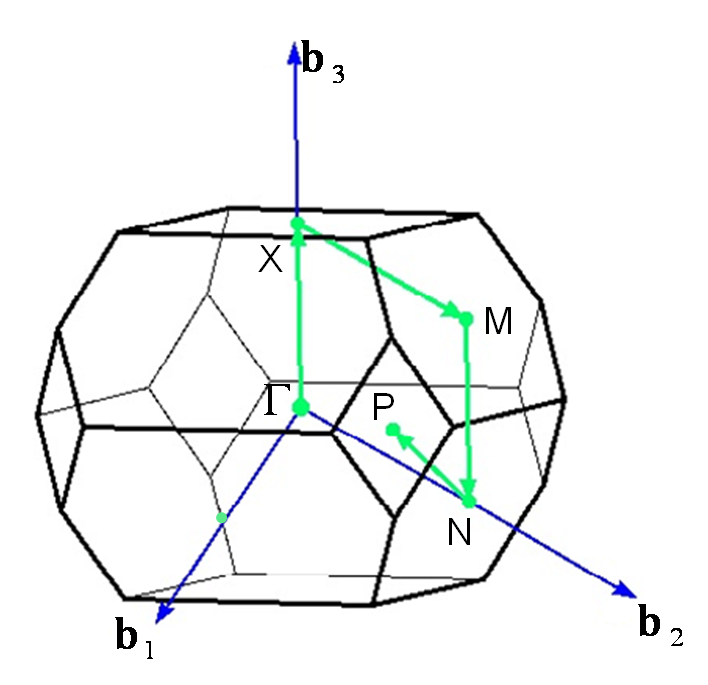
\includegraphics[height=50mm]{bz.eps}
\caption{The first Brillouin zone of CIGS}
\end{center}
\end{figure}

\noindent The first Brillouin Zone (BZ) is the Wigner-Seitz primitive cell in reciprocal space, for example, the figure \ref{bz} is the first BZ of CIGS, where $\textbf{b}_1$, 
$\textbf{b}_2$ and $\textbf{b}_3$ are reciprocal lattice basis vectors. The following is the table about high symmetry points of the first BZ.


%\FloatBarrier
\vspace{10cm}


\begin{table}{}
\begin{center}
\begin{tabular}{|c|c|c|c|}
  \hline
  \multicolumn{4}{ | r |}{Points Coordinates($\textbf{b}_1$,$\textbf{b}_2$,$\textbf{b}_3$)} \\
  \hline
  $\Gamma$ & 0 & 0 & 0 \\
    \hline
   X & 0 & 0 & 1/2 \\
   \hline
   M & 0 & 1/2 & 1/2 \\
   \hline
   N & 0 & 1/2 & 0 \\
   \hline
   P & 1/2 & 1/2 & 1/2 \\
  \hline
\end{tabular}
\caption{\textit{High Symmetry Points of BZ for CIGS}}
\end{center}
\end{table}



\section{Band structure and density of state}
\noindent In solid, there are huge amount of atoms which interact each other, so the discrete of energy split into the huge number of state
 with small difference, those are defined as energy band, it is very important if we want to know more about electrons or optical
 properties. So the band structure of CIGS is given as follows:

\begin{figure}[h]\label{bs}
\begin{center}
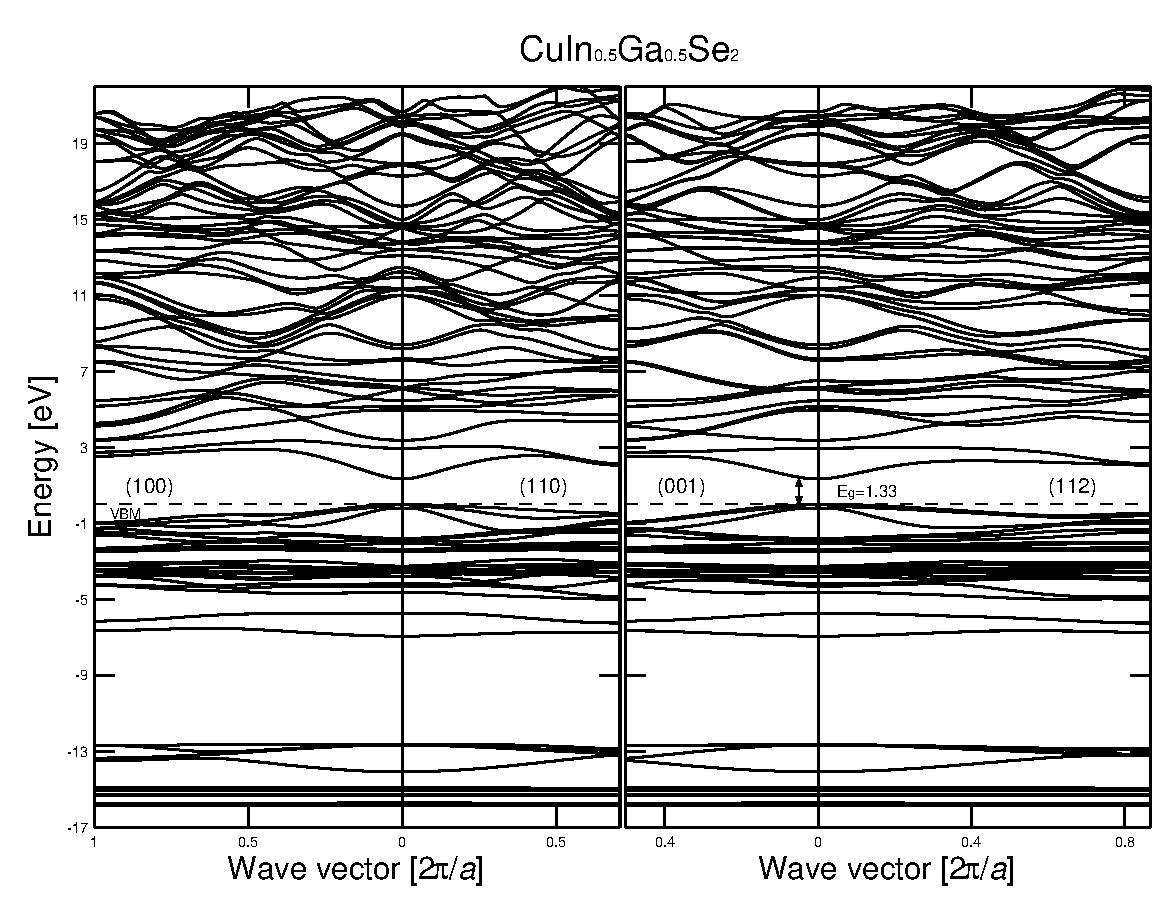
\includegraphics[height=90mm, width=110mm]{bandstr_theis.eps}
\caption{The band structure of CIGS}
\end{center}
\end{figure}

\noindent The density of states (DOS) of a system is the number of states which could be occupied per interval of energy. And the DOS of CIGS is: 

{\color{red}??????????????????? add DOS figure ?????????????????????????} 





\chapter{FP-LAPW method}
\section{Introduction}
\noindent So far, We already know how to solve the Kohn-Sham equation, however, there are still two more questions in the air, what is the exact form of 
wavefunction and potential in the realistical calculation ?  

\noindent One maybe naturally choose the a set of plane waves as wavefunction because of bloch theory, but there is a drawback about the plane wave 
when discribing the nearby the atomic core region, because the wavefunction change dramatically, so one needs to choose more plane
waves to define it, which means it will take more time to calculate.

\noindent Slater re-consider the way to discribe the wavefunction, he splits the unit cell into two regions, one is the sphere region which is
defined by the center of atom, but non-overlap each sphere, called muffin tin (MT) region, the remaining region is called interstitial 
(I) region. And an atomic like function is defined as the wavefunction in MT region, this is reason why the method is called augmented plane wave (APW),
 and in the interstitial region wavefunction is discribed as plane wave, which is reasonable, because the wave 
function approaching atomic core is somehow like inside atom, but far away the atomic core, the electron behaves like free electrons,
 so plane wave is suitable. However, the drawback of APW method is the wavefunction is dependent with the energy, which leads to the 
nonlinear eigenvalue problem, so in order to get the exact energy, the method have to decide repeatlly, which is really time-consumming.
%%%%%%%%%%%%%%%%% figure of mf and ir
\noindent In order to find a way out, is it possible to let the wavefunction energy-independent?, Andesen and Koelling and Arbman?? proposes a way to discribe that, he notices that
the taylor expansion of radial function, and make use of it to linearize the APW method, so the method is called Linearized Augmented Plane Wave (LAPW) method.
However, the drawback is that this method does not discribe the core state well, so the method is corrected by method of LAPW+LO and LAPW+lo, which is proposed by ?? and ?? respectively.

{\color{red}??????????????????? need to understant more about LAPW+LO and +lo ?????????????????????????} 


\section{Augmented Plane Wave method}
\noindent Slater defines the wavefunction like the following equation:
\begin{comment}
\begin{equation*}\label{ap1}
\phi^{APW}_\textbf{k+G} (\textbf{r})= 
\begin{cases} \frac {1}{\sqrt{\Omega}} e^{i(\textbf{k+G})\textbf{r}} & \quad \mbox{if $\textbf{r} \in I, $}
\\
\sumg<\alpha>\sum\limits_{{\ell}m} f_{{\ell}{m}} (r_{\alpha},\textbf{k+G} E) Y_{{\ell}m}(\hat{\textbf{r}}_{\alpha})  & \quad \mbox{if $\textbf{r} \in S_\alpha, $}\\ 
\end{cases}
\end{equation*}

where $f_{{\ell}{m}} (r_{\alpha},\textbf{k+G} E) = \sum\limits_{q=1}^{M_{\ell}^{\alpha}} A _{q{\ell}m}^{\alpha}\bf(k+G) u_{q{\ell}}^{\alpha}(r, E)$

$A _{q{\ell}m}^{\alpha}\bf(k+G)$ is the expasion coefficients, and $u_{q{\ell}}^{\alpha}(r, E)$  is the radial function, which is dependent with energy $E$, and the
radial function could be decided by the following equation:
\end{comment}

\begin{equation*}\label{ap1}
\phi^{APW}_\textbf{k+G} (\textbf{r})= 
\begin{cases} \frac {1}{\sqrt{\Omega}} e^{i(\textbf{k+G})\textbf{r}} & \quad \mbox{if $\textbf{r} \in I, $}
\\
\sumg<\alpha>\sum\limits_{{\ell}m} f_{{\ell}{m}} (r_{\alpha},\textbf{k+G}, E) Y_{{\ell}m}(\hat{\textbf{r}}_{\alpha})  & \quad \mbox{if $\textbf{r} \in S_\alpha, $}\\ 
\end{cases}
\end{equation*}

\noindent where $f_{{\ell}{m}} (r_{\alpha},\textbf{k+G} ,E) =  A _{{\ell}m}^{\alpha} \bf(k+G) u_{{\ell}}^{\alpha}(r_{\alpha}, E)$ and $A _{{\ell}m}^{\alpha} \bf(k+G) $is the expasion coefficients, and $u_{{\ell}}^{\alpha} (r_{\alpha}, E)$  is the radial function, which is dependent with energy $E$, and the
radial function could be decided by the following:
\begin{equation}\label{ap2}
(-\frac{1}{2} \frac{d^2}{dr_{\alpha}^2} + \frac{\ell(\ell+1)}{2r_{\alpha}^2}+V(r_{\alpha})-E)r_{\alpha}u_{\ell}(r_{\alpha}) = 0
\end{equation}

\noindent where $V(r_{\alpha})$ is the spherical potential. The following is the figure about this basis function

%%%%%%%%%%%%%%%%%%%%%%  figure mt and interstial region

\noindent Because wavefunction has dual representations, one has to make sure the continousiny on the sphere, which is solved by matching each $\ell m$
of the dual representation.

{\color{red}??????????????????? add the representations figure of basis function ?????????????????????????} 


\noindent from the above figure, $\bf{r=R^{\alpha}+r_{\alpha}}$ is guaranteed. so taking use of the Rayleigh expansion formula:
\begin{equation}
\expg<(k+G)>= e^{i \textbf(k+G) \textbf{R}^{\alpha} } 4 \pi \sumlm<\ell><m> i^{\ell} \bessf< |\bf{k+G}|> \sphfr<\ell{m}><r><> \sphfq<\ell{m}><\textbf{k+G}><*>
\end{equation}
  
\noindent after matching those two representations, the following equation is satisfied:

\begin{equation}
A _{{\ell}m}^{\alpha} \bf(k+G)= \frac{ e^{i \textbf(k+G) \textbf{R}^{\alpha} } 4 \pi \sumlm<\ell><m> i^{\ell} \bessf< |\bf{k+G}|> \sphfq<\ell{m}><\textbf{k+G}><*> }{\sqrt{\Omega} u_{{\ell}}^{\alpha}(r_{\alpha}, E)}
\end{equation}

\noindent There are two main drawbacks about the APW method:
The first one is that the wavefuntion is energy dependent, which means that the code will search for the energy in order to calculate the exact energy, so it 
is really time consumming.The second one the less harmful, but also sometimes it will cause problem when $u_{{\ell}}^{\alpha}(r_{\alpha}, E) = 0$ during matching. 

\section{Linearized Augmented Plane Wave method}
\noindent In order to decouple the energy and wavefunction, Andersson finds out a way to seperate them, he notices that the taylor expansion of the radail function
on certain energy, which can be expressed as follows:

\begin{equation}
 u_{{\ell}}^{\alpha}(r_{\alpha}, E) = u_{{\ell}}^{\alpha}(r_{\alpha}, E_{\ell}) + (E-E_{\ell}) \dot{u}_{{\ell}}^{\alpha}(r_{\alpha}, E_{\ell})
\end{equation}

\noindent So he re-defines the wavefuntion in the following way:

\begin{equation*}\label{lap1}
\phi^{LAPW}_\textbf{k+G} (\textbf{r})= 
\begin{cases} \frac {1}{\sqrt{\Omega}} e^{i(\textbf{k+G})\textbf{r}} & \quad \mbox{if $\textbf{r} \in I, $}
\\
\sumg<\alpha>\sum\limits_{{\ell}m} f_{{\ell}{m}} (r_{\alpha},\textbf{k+G}, E_{\ell}) Y_{{\ell}m}(\hat{\textbf{r}}_{\alpha})  & \quad \mbox{if $\textbf{r} \in S_\alpha, $}\\ 
\end{cases}
\end{equation*}

\noindent where $f_{{\ell}{m}} (r_{\alpha},\textbf{k+G} ,E_{\ell}) =  A _{{\ell}m}^{\alpha} \bf(k+G) u_{{\ell}}^{\alpha}(r_{\alpha}, E_{\ell}) + B _{{\ell}m}^{\alpha} \bf(k+G) \dot{u}_{{\ell}}^{\alpha}(r_{\alpha}, E_{\ell})$
$A _{{\ell}m}^{\alpha} \bf(k+G)$ and $B _{{\ell}m}^{\alpha} \bf(k+G)$ is the expansion coefficients, and $\dot{u}_{{\ell}}^{\alpha}(r_{\alpha}, E_{\ell}$ is the derivate of the radial function.

\noindent Here energy $E_{\ell}$  is considered as pre-calculated parameter, actually, it is chosen by the middle of  each l-character band.

\noindent Apparently, LAPW method is more suitable in reality, because the wavefunction is decoupled with energy, but it has to match for two parameters,
fortunaly, even though, it still use less time comparing with APW method. However, there is one drawbacks, what if energy difference is big in the same $ {\ell} $ charater, 
which the $E_{\ell}$ is correct, so this situation will cause big error, these states are called as semi-core state, for example, the alkali metal, the actinides and the rare earths and so on.

\section{Linearized Augmented Plane Wave method + LO}
Comparing with LAPW method, LAPW+LO method extend the basis set, and add smaller number of basis set, which has the following format:


\begin{equation*}\label{lap1}
\phi^{LO}_\textbf{k+G} (\textbf{r})= 
\begin{cases} 0 & \quad \mbox{if $\textbf{r} \in I, $}
\\
(A _{{\ell}m}^{\alpha}  u_{{\ell}}^{\alpha}(r_{\alpha}, E_{\ell}) + B _{{\ell}m}^{\alpha}  \dot{u}_{{\ell}}^{\alpha}(r_{\alpha}, E_{\ell}) + C _{{\ell}m}^{\alpha}  u_{{\ell}}^{\alpha}(r_{\alpha}, E^{\prime}_{\ell})){Y_{{\ell}m}(\hat{\textbf{r}}_{\alpha})} & \quad \mbox{if $\textbf{r} \in S_\alpha, $}\\ 
\end{cases}
\end{equation*}
 
where $A _{{\ell}m}^{\alpha}$ and $B _{{\ell}m}^{\alpha}$ is matching value and derivate on the sphere boundary to zero, but not plane wave, like LAPW did before, and $E^{\prime}_{\ell}$ is
the chosen energy from semi-core state.

\section{Augmented Plane Wave method plus local orbitals}
Actually, there is one more method which will deal with the energy-denpendent case, which is called as Augmented Plane Wave method plus local orbitals (APW+lo), the 
basis function has two kinds, one is similar with equation \ref{lap1}, but only without the derivative terms, e.g., $f_{{\ell}{m}} (r_{\alpha},\textbf{k+G} ,E_{\ell}) =  A _{{\ell}m}^{\alpha} \bf(k+G) u_{{\ell}}^{\alpha}(r_{\alpha}, E_{\ell})$.
And another basis function is:
\begin{equation*}\label{lap3}
\phi^{lo}_\textbf{k+G} (\textbf{r})= 
\begin{cases} 0 & \quad \mbox{if $\textbf{r} \in I, $}
\\
(A _{{\ell}m,lo}^{\alpha}  u_{{\ell}}^{\alpha}(r_{\alpha}, E_{\ell}) + B _{{\ell}m,lo}^{\alpha}  \dot{u}_{{\ell}}^{\alpha}(r_{\alpha}, E_{\ell}) ){Y_{{\ell}m}(\hat{\textbf{r}}_{\alpha})} & \quad \mbox{if $\textbf{r} \in S_\alpha, $}\\ 
\end{cases}
\end{equation*}
 
And the value of $A _{{\ell}m,lo}^{\alpha}$ and $B _{{\ell}m,lo}^{\alpha}$ are obtained by normalization and local orbital has zero value at the muffin tin boundary.

\chapter{K $\cdot$ P method}

The basic idea will be explained in the following text. First, from Bloch Theory we know 

\begin{equation}\label{1}
 \wfbloch<n><k> = \expg<k> \ubloch<n><k>
\end{equation}

where $\wfbloch<n><k>$ is the wave function on k point for the {\it n}th band, and $\expg<k>$ is plane wave, $\ubloch<n><k>$ is a function which has the same a periodicity as the potential.





Now let us suppose we already got the wavefunction and energy by some procedure on $k_0$ point, $\wfbloch<n><k_0>$ is the wavefunction and $\ebloch<n><k_0>$ is the energy.
We define another function as the following:

\begin{equation}\label{2}
\chikp<n><k> = \expg<(k-k_0)> \wfbloch<n><k_0>
\end{equation}





 we can expand the above function $\chikp<n><k> $ as wave function on $k$ point, and then we can calculate the wave function on the $k$ point.
\begin{equation}\label{3}
\wfbloch<n><k> =  {\sum\limits_{\color{red} j}} C_{n,j}^{k} \chikp<n><k> 
\end{equation}



From above equation, we will know the wave function if we get the coefficient $C_{n,j}^{k}$, let us substitute the equation \ref{3} into Kohn-Sham equation.
\begin{equation}\label{4}
\left\{ \frac {{\bf p}^2} {2m} + V({\bf r}) \right\} \wfbloch<n><k> = \ebloch<n><k> \wfbloch<n><k>
\end{equation} 






then we will finally get the following equation.
\begin{equation}\label{5}
{\sum\limits_{j}}  C_{n,j}^{k} \left \{  \left [  \ebloch<j><k_0> -  \ebloch<n><k>  + \frac{{\hbar}^2}{2m} {\bf (k^2-k_0^2)}    \right ] \delta_{j',j} + \frac{\hbar}{m} {\bf(k-k_0)} {\bf p_{j',j}} \right \} = 0
\end{equation}

where ${\bf p_{j',j}} = \langle \ubloch<j'><k_0>| {\bf p} | \ubloch<j><k_0>  \rangle $.
 
We also can simpify the above equation in the following format:
\begin{equation}\label{6}
{\sum\limits_{j}} C_{n,j}^{k} \left \{ H_{j',j}- \ebloch<n><k> \delta_{j',j} \right \} =0
\end{equation}

where $H_{j',j} = \left [  \ebloch<j><k_0>  + \frac{{\hbar}^2}{2m} {\bf (k^2-k_0^2)}    \right ] \delta_{j',j} + \frac{\hbar}{m} {\bf(k-k_0)} {\bf p_{j',j}}$, from the above equation, we 
can calculate the coefficient $ C_{n,j}^{k}$.




\chapter{Scalar relativistic approximation and the spin orbit coupling}
\label{ch:dft}

\section{Dirac equation}


\noindent Non-relativistic quantum mechanics has broad application, but when the speed of electron is near the speed of light, 
the non-relativistic quantum is not suitable to describe the system of electron. So Dirac introduced an equation which is called
Dirac equation applying for relativistic case.

\noindent Dirac defined the Hamiltonian: 


\begin{equation}\label{dirac}
\hat{H}_\textit{dirac} = c \boldsymbol{\alpha} \textbf{P} + \boldsymbol{\beta}mc^{2} + V
\end{equation}

\noindent where $\textbf{P} = -i\hbar \nabla $ is the momentum operator,$V$ is the general potential(??????? Defined in KS), $m$ is the mass of electron 
and $c$ is the speed of light, $\boldsymbol{\alpha}$ and $\boldsymbol{\beta}$ are $4 \times 4$ matrices.
\begin{equation}
 \boldsymbol{\alpha} = \left( \begin{array}{cc}
 0 & \boldsymbol{\sigma}  \\
 \boldsymbol{\sigma} & 0   \end{array} \right),
\boldsymbol{\beta}= \left( \begin{array}{ccc}
\boldsymbol{I} & 0\\
0 & -\boldsymbol{I}\end{array} \right)
\end{equation}

\noindent where $\boldsymbol{I}$ is unit matrix, and $\boldsymbol{\sigma}$ is Pauli matrix.

\begin{equation} 
\boldsymbol{\sigma} = (\boldsymbol{\sigma}_x \  \boldsymbol{\sigma}_y \  \boldsymbol{\sigma}_z )  
\end{equation}

\begin{equation}
\boldsymbol{\sigma}_x= \left( \begin{array}{cc}
0 & 1\\
1 & 0\end{array} \right),
\boldsymbol{\sigma}_y= \left( \begin{array}{ccc}
0 & -i\\
i & 0\end{array} \right),
\boldsymbol{\sigma}_z= \left( \begin{array}{ccc}
1 & 0\\
0 & -1\end{array} \right)
\end{equation}




\section{Derivation of scalar relativistic approximation and the spin orbit coupling}

\noindent  $\Psi$ is the wavefunction of Hamiltonian \ref{dirac}, which has four components, but can be 
written with only two terms:
\begin{equation}\label{diracwf}
\Psi= \left( \begin{array}{c}
\phi^{\uparrow} \\
\phi^{\downarrow} \\
\chi^{\uparrow} \\
\chi^{\downarrow} \end{array} \right),
 \Psi = \left(\begin{array}{c}
\phi \\               
\chi \end{array} \right)
\end{equation}


\noindent where $\phi$ includes the two terms of $\phi^{\uparrow}$ and $\phi^{\downarrow}$, and $\chi$ contains  $\chi^{\uparrow}$ and $\chi^{\downarrow}$;
under the nonrelativistic limit,$\phi$ is bigger than $\chi$ by the ratio of $v/c$, where $v$ and $c$ are speed of particle and light, respectively,
so the $\phi$ is the large term and $\chi$ is the small one.

\noindent In order to derive the scalar relativistic approximation and the spin-orbit coupling terms, we need to take use of the nonrelativistic limit approximation of the 
Dirac eigenvalue equation probelm, here nonrelativistic limit means $v^2/c^2 << 1$.

\begin{equation}\label{diracse}
 E \Psi = (c \boldsymbol{\alpha} \textbf{P} + \boldsymbol{\beta}mc^{2} + V) \Psi
\end{equation}

\noindent For convenience, we define:

\begin{equation}\label{dirace}
E^{\prime} = E - mc^2
\end{equation}

\noindent where $E$ is the total energy, $mc^2$ are $E'$ are the rest mass energy and the remaining energy excluding the rest mass energy, under the nonrelativistic limit, 
$E'$ is far smaller than $mc^2$. Now, putting equation \ref{diracwf} and \ref{dirace} into equation \ref{diracse}:

\begin{equation}
\begin{split}
&(E^{\prime} - V) \Phi - c \boldsymbol{\sigma} \textbf{P} \chi = 0\\                
&-c\boldsymbol{\sigma} \textbf{P} \Phi + (E^{\prime}+2mc^2-V)\chi = 0
\end{split}
\end{equation}

\noindent To eliminate the $\chi$ (otherwise, it is the antiparticle problem), we can end up with the equation:
  \begin{equation}
(V + \frac{1}{2m} (\boldsymbol{\sigma} \textbf{P}) (1+\frac{E^{\prime}-V}{2mc^2})^{-1} (\boldsymbol{\sigma} \textbf{P}) )\phi=E^{\prime}\phi
\end{equation}

\noindent Since ${E^{\prime}-V}$ is far smaller than ${2mc^2}$, so taking advantage of the taylor expansion and the following identites:
\begin{equation}
\begin{split}
& [\textbf{P}, V ]= -i \hbar \triangledown V \\                
&(\boldsymbol{\sigma} \textbf{A} )(\boldsymbol{\sigma} \textbf{B}) = \textbf{A} \textbf{B} + i\boldsymbol{\sigma}[\textbf{A} \times \textbf{B}]
\end{split}
\end{equation}


\noindent After some operations, we finally will get the following equation under the nonrelativistic limit:

\begin{equation}
E^{\prime} \phi = (\frac{\textbf{P}^2}{2m} + V - \frac{\textbf{P}^4}{8 {m}^3 {c}^2}-\frac{i\hbar}{4{m}^2 {c}^2} (\nabla{V})\textbf{P}+\frac{\hbar}{4 m^2 c^2} \boldsymbol{\sigma}[\nabla{V} \times \textbf{P}]) \phi
\end{equation}


\noindent Furthermore, we can approximate the above equation to the simpler expression under spherical symmetry potential:

\begin{equation}
 E^{\prime} \phi = (\frac{\textbf{P}^2}{2m} +V - \frac{\textbf{P}^4}{8 {m}^3 {c}^2}-\frac{i\hbar}{4{m}^2 {c}^2} (\nabla{V})\textbf{P}+\frac{1}{2 m^2 c^2} \frac{1}{R} \frac{dV}{dR}\textbf{S}\textbf{L}) \phi
\end{equation}

\noindent where $\textbf{S}={\hbar}{\boldsymbol{\sigma}}/2$ is the Pauli spinor, and $\textbf{L}=\textbf{R} \times \textbf{P}$ is the orbital
angular momentum operator. The terms of ${\textbf{P}^2}/(2m) + V$ is Schrödinger term,  ${\textbf{P}^4}/(8 {m}^3 {c}^2)$ and ${i\hbar} (\nabla{V})\textbf{P} /(4{m}^2 {c}^2)$  are the mass enhancement 
and Darwin term, respectively, both of them together is called the scalar relativistic approximation (SRA), the last term is the spin-orbit coupling(SOC) term.


\section{Implementation of scalar relativistic approximation and spin-orbit coupling}
\noindent In this section, we will focus on the implementation of scalar relativistic approximation and spin-orbit coupling in the Exciting Code,
and we have to point out, the implementation is done only in the interstitial region(details see the introduction in the FP-LAPW method on page ???), 
the most important part from the  implementation point is the matrix element, so first we will derive the matrix element of SRA, and then SOC, at last,
we take use of different approaches to test the accuracy of the implementation.

\subsection{Matrix element for the scalar relativistic approximation }
\noindent To calculate the scalar relativistic approximation affect in the interstitial region, we need to fomulate matrix element of SRA, first we define the \hm  of SRA:

\begin{equation}
\begin{split}
 & \widehat{H}_{sra} = - \frac{\textbf{P}^4}{8 {m}^3 {c}^2} -\frac{i\hbar}{4{m}^2 {c}^2} (\nabla{V})\textbf{P} \\
 & = -\frac{\hbar^4 \nabla^4}{8{m}^3 {c}^2} - \frac{\hbar^2}{4m^2c^2}(\nabla{V})\nabla
\end{split}
\end{equation}

\noindent In the atomic unit, we can simplify the above equation:
\begin{equation}
  \widehat{H}_{sra} =  -\frac{\nabla^4}{8 {c}^2} - \frac{(\nabla{V})\nabla}{4 c^2}
\end{equation}

\noindent The matrix element can be expressed:

\begin{equation}
\begin{split}
& H_{G,G'}^{sra} = < \phi_G | \widehat{H}_{sra}  | \phi_{G'} >  \\
&  = \frac{1}{\Omega} < \expg<(k+G)> |  -\frac{\nabla^4}{8 {c}^2} - \frac{(\nabla{V})\nabla}{4 c^2} |  \expg<(k+G')>>  \\
&  = \frac{1}{8 {c}^2 \Omega} \int_{I} d \textbf {r} \expg<(G'-G)> \{-(k+G)^2(k+G')^2 -2i(k+G') \sumg<G''> V_{G''}iG'' \expg<G''>\}  \\
&  =  \frac{1}{8 {c}^2 \Omega} \int_{I} d \textbf {r} \expg<(G'-G)> \{-(k+G)^2(k+G')^2 + 2(k+G') \sumg<G''> V_{G''}G'' \expg<G''>\}  
\end{split}
\end{equation}


\noindent Splitting two terms from the above equation, the first term is :
\begin{equation}\label{sra1}
\begin{split}
&  H_{1}^{sra} = \frac{1}{8 {c}^2 \Omega} \int_{I} d \textbf {r} \expg<(G'-G)> \{-(k+G)^2(k+G')^2\}  \\
&  = \frac{-(k+G)^2(k+G')^2}{8 {c}^2 } \frac{1}{\Omega} \int_{I} d \textbf {r} \expg<(G-G')>   \\
&  = \frac{-(k+G)^2(k+G')^2}{8 {c}^2 } \frac{1}{\Omega} \int_{\Omega} d  \textbf {r} \expg<(G'-G)> \theta_{I}(r)  \\
&  = \frac{-(k+G)^2(k+G')^2}{8 {c}^2 } \widetilde{\theta}_{I}(G-G')  \\
\end{split}
\end{equation}

\noindent where $\theta_{I}(r)$ is the characteristic function of the interstitial region ( $r$ included in MT, $\theta_{I}(r)$ = 0, otherwise it is 1), $\widetilde{\theta}_{I}(r)$ comes from the Fourier transform of $\theta_{I}(r)$:
\begin{equation}
\theta_{I}(r) = \sumg<G> \widetilde{\theta}_{I}(G) \expg<G>
\end{equation}

\noindent And
 
\begin{equation*}\label{ap1}
\widetilde{\theta}_{I}(G) =
\begin{cases}  \delta_{G,0}-\sumg<\alpha> \frac{4 \pi R_{\alpha}^{3}}{\Omega} \frac{j_1(|G|R_{\alpha})}{|G|R_{\alpha}} e^{-iGr_{\alpha}} & \quad \mbox{if $\textbf{G} \leqslant \textbf{G}_{max} $}
\\
0  & \quad \mbox{if $\textbf{G} > \textbf{G}_{max} $}\\ 
\end{cases}
\end{equation*}

\noindent where $R_{\alpha}$ is the radius of the MT, $r_{\alpha}$ is the position refer to the $\alpha$th atom, and $j_1$ is the $\it1$st order Bessel function.

T\noindent he second term is:
\begin{equation}\label{sra2}
\begin{split}
& H_{2}^{sra} = \frac{2(k+G') \sumg<G''> V_{G''}G''}{8 {c}^2 \Omega} \int_{I} d \textbf {r} \expg<(G'-G)>  \expg<G''>  \\
& =  \frac{(k+G') \sumg<G''> V_{G''}G''}{4 {c}^2 } \frac{1}{\Omega} \int_{I} d \textbf {r} \expg<(G'-G+G'')>  \\
& =  \frac{(k+G') \sumg<G''> V_{G''}G''}{4 {c}^2 } \widetilde{\theta}_{I}(G-G'-G'')
\end{split}
\end{equation}

\noindent So finally, after joining the equation \ref{sra1} and \ref{sra2} together, the final matrix element for the scalar relativistic approximation is:
\begin{equation}\label{sra4}
\begin{split}
 & H_{G,G'}^{sra} = \frac{1}{{8 {c}^2 }} \{ -(k+G)^2(k+G')^2 \widetilde{\theta}_{I}(G-G') \\
 & + 2{(k+G') \sumg<G''> V_{G''}G''} \widetilde{\theta}_{I}(G-G'-G'') \}
\end{split}
\end{equation}




\subsection{Matrix element for the spin-orbit coupling }
\noindent The spin-orbit coupling is included in second-variational scheme for the Exciting code, 
\noindent  which means it takes use of the basis function which is expanded from the first variational wavefunction.
\begin{equation}
\begin{split}
 & \widehat{H}_{1}   \phi^{i}_{1}  = E^{i}_1  \phi^{i}_{1} \\
 & (\widehat{H}_1+\widehat{H}_{soc})  \Psi  = E \Psi
\end{split}
\end{equation}
\noindent  where $ \widehat{H}_{1}$ and $ \phi^{i}_{1}$ are first variational \hm and wavefunction, respectively, and $\Psi = \sumi<i> c_{i} \phi^{i}_1$.
If  multiply $\phi^{j}_{1}$ on the left side of the second item of the above equation.
\begin{equation}
\begin{split}
 & <  \phi^{j}_1 |(\widehat{H}_1+\widehat{H}_{soc}) | \sumi<i> c_{i} \phi^{i}_1 > = E< \phi^{j}_1 | \sumi<i> c_{i} \phi^{i}_1>
\end{split}
\end{equation}

\noindent After some operations, the above equation becomes:
\begin{equation}
\begin{split}
 &\sumi<i> c_{i} \{ E^{i}_{1} \delta_{i,j} +<\phi^{j}_1 |\widehat{H}_{soc} | \phi^{i}_1  > \} = \sumi<i> c_{i} E \delta_{i,j}
\end{split}
\end{equation}
 
\noindent So finally, the above equation becomes the eigenvalue probelm $H_2 C = E C$.
\begin{equation}\label{ep4}
H_2=\left[
\begin{matrix}
    E_1+H_{11} & H_{12} & \cdots & H_{1N} \\
    H_{21} & E_2 + H_{22} & \cdots & H_{2N} \\
    \vdots               & \vdots               &        & \vdots               \\
     H_{N1} & H_{N2} & \cdots & E_{N}+H_{NN} \\
\end{matrix} \right],
C = \left[ \begin{array}{c} C_1 \\ C_2 \\ \vdots \\ C_N\end{array} \right]
\end{equation}

\noindent where $H_{j,i} = <\phi^{j}_1 |\widehat{H}_{soc} | \phi^{i}_1  > $. Actually, each block matrix of equation \ref{block} is similar with above matrix 
for the implementation in the Exciting code,since there are spin up and spin down combinations. 

\noindent  To formulate the matrix element for SOC, first we define the \hm term of SOC:
\begin{equation}
\begin{split}
 & \widehat{H}_{soc} = \frac{-i\hbar^2}{4m^2c^2} \boldsymbol{\sigma} [ (\triangledown V) \times \triangledown]
\end{split}
\end{equation}

\noindent Converting the above equation to atomic unit:

\begin{equation}
\begin{split}
 & \widehat{H}_{soc} = \frac{-i}{4 c^2} \boldsymbol{\sigma} [ (\triangledown V) \times \triangledown]
\end{split}
\end{equation}

\noindent Now calculate the matrix element:

\begin{equation}\label{soc}
\begin{split}
& H_{j,j'}^{soc} = < \Psi_j | \widehat{H}_{soc}  | \Psi_{j'} >  \\
& =   < \sumg<G> c_{j,k+G} \expg<(k+G)>  |  \frac{-i}{4 c^2} \boldsymbol{\sigma} [ (\triangledown V) \times \triangledown] |  \sumg<G'> c_{j',k+G'} \expg<(k+G')> > \\
& = \frac{i}{4c^2}\sumg<G,G',G''> c_{j,k+G}^{*} c_{j',k+G'} V_{G''} < \expg<(k+G)> | \expg<(k+G'+G'')>   \left( \begin{array}{cc}
h_z & h_x-i h_y\\
h_x+i h_y & -h_z\end{array} \right) > \\
& =  \frac{i}{4c^2}\sumg<G,G',G''> c_{j,k+G}^{*} c_{j',k+G'} V_{G''}  \left( \begin{array}{cc}
h_z & h_x-i h_y\\
h_x+i h_y & -h_z\end{array} \right)  \int_{I} \expg<(G'+G''-G)>   \\
& = \frac{i}{4c^2}\sumg<G,G',G''> c_{j,k+G}^{*} c_{j',k+G'} V_{G''}  \left( \begin{array}{cc}
h_z & h_x-i h_y\\
h_x+i h_y & -h_z\end{array} \right)  \widetilde{\theta}_{I}(G-G'-G'')  
\end{split}
\end{equation}

\noindent where $ c_{j,k+G}$ is the eigenvector from the first variational scheme, and $h_x$, $h_y$ and $h_z$ are the three components of the $h$:
\begin{equation}
 h=h(k,G',G'')= G'' \times (k+G')
\end{equation}

\noindent So in the subroutine of Exicting Code, the \hm is divided by the 2 $\times$ 2 matrix,
 each block of the matrix means the spin up and down combination matrix:

\begin{equation}\label{block}
 \left( \begin{array}{cc}
\uparrow \uparrow & \uparrow \downarrow\\
\downarrow \uparrow & \downarrow \downarrow \end{array} \right)
\rightarrow \left( \begin{array}{ccc}
h_z & h_x-ih_y\\
h_x+ih_y & -h_z\end{array} \right)
\end{equation}

\noindent where $\downarrow$ and $\uparrow$ represent spin down and up, respectively. 
\noindent For example, when we calculate $\uparrow \uparrow $ part of the matrix,the equation \ref{soc} becomes: 
\begin{equation}\label{soc2}
\begin{split}
& H_{j,j'}^{soc} = \frac{i}{4c^2}\sumg<G,G',G''> c_{j,k+G}^{*} c_{j',k+G'} V_{G''}  h_z  \widetilde{\theta}_{I}(G-G'-G'')  
\end{split}
\end{equation}
 If the $\downarrow \downarrow $ part of the matrix,the equation \ref{soc} becomes:
\begin{equation}
\begin{split}
& H_{j,j'}^{soc} = \frac{i}{4c^2}\sumg<G,G',G''> c_{j,k+G}^{*} c_{j',k+G'} V_{G''} (- h_z)  \widetilde{\theta}_{I}(G-G'-G'')  
\end{split}
\end{equation}
 If the $\uparrow \downarrow $ part of the matrix,the equation \ref{soc} becomes:
\begin{equation}\label{soc3}
\begin{split}
& H_{j,j'}^{soc} = \frac{i}{4c^2}\sumg<G,G',G''> c_{j,k+G}^{*} c_{j',k+G'} V_{G''} (h_x-i h_y)  \widetilde{\theta}_{I}(G-G'-G'')  
\end{split}
\end{equation}



\section{Test of scalar relativistic approximation and spin-orbit coupling}
In order to test the affect of SRA and SOC, It is not that easy job since the SOC and SRA is implemented in the IR, but still, we can search for some points to 
test the validity of SRA and SOC, in the next subsection, I will show the test from the different derivation and concrete example as well.

\subsection{Test of matrix element for the scalar relativistic approximation }
\noindent To test the SRA affect, I am still looking for concrete example from the application point, but from the theoretical point,
I can use different mathmatical derivation to implement the code, and compare the accuracy.

\noindent So there is another point derivation from the SRA \hm, the equation \ref{sra1} is still the same, but the second term:

\begin{equation}\label{sra3}
\begin{split}
&  H^{2}_{sra} = \frac{1}{\Omega} < \expg<(k+G)> |  -\frac{(\nabla{V(r)})\nabla}{4 c^2} |  \expg<(k+G')>>  \\
&  = \frac{-1}{4 {c}^2 \Omega} \int_{\Omega} d \textbf {r} e^{-i(k+G)} \{ {\theta}_{I}(r) \nabla{V(r)}    i(k+G')  \expg<(k+G')>\}  \\
&  =  \frac{-i(k+G')}{4 {c}^2 \Omega} \int_{\Omega} d \textbf {r} e^{-i(k+G)} \{ {\theta}_{I}(r) \nabla{V(r) }     \expg<(k+G')>\}  \\
\end{split}
\end{equation}

\noindent In the above equation,  we take advantage of the Fourier transform:
\begin{equation}
 {\theta}_{I}(r) \nabla{V(r )} = \sumg<G''> \widetilde{V}_{G''} \expg<G''>
\end{equation}

\noindent Then the equation \ref{sra3} will change to :
\begin{equation}\label{sra6}
\begin{split}
&  H_{2}^{sra} = = \frac{-i(k+G')}{4 {c}^2 \Omega} \int_{\Omega} d \textbf {r} e^{-i(k+G)} \{ {\theta}_{I}(r) \nabla{V(r) }     \expg<(k+G')>\}  \\
& = \frac{-i(k+G')}{4 {c}^2 \Omega} \int_{\Omega} d \textbf {r} \sumg<G''> \widetilde{V}_{G''}  e^{i(G'-G+G'')} \\
& =  \frac{-i(k+G')}{4 {c}^2 } \sumg<G''> \widetilde{V}_{G''} \delta_{G'',G-G'} \\
& = \frac{-i(k+G')}{4 {c}^2 } \widetilde{V}_{G-G'}
\end{split}
\end{equation}

\noindent So finally, we get the final equation:
\begin{equation}\label{sra5}
\begin{split}
 & H_{G,G'}^{sra} = \frac{-(k+G)^2(k+G')^2}{8 {c}^2 } \widetilde{\theta}_{I}(G-G')  +  \frac{-i(k+G')}{4 {c}^2 } \widetilde{V}_{G-G'}
\end{split}
\end{equation}

\noindent Comparing equation \ref{sra4} with equation \ref{sra5}, actually, the code will get more performance when using the equation \ref{sra5} since the $G''$ 
normally is in the order of $10^4$ to $10^5$.

\noindent Now we compare these two methods with the calculated matrix element value.   



\begin{figure}[ht!]
     \begin{center}
        \subfigure[rgkmx=7, gmaxvr=7]{%
            \label{fig:first}
            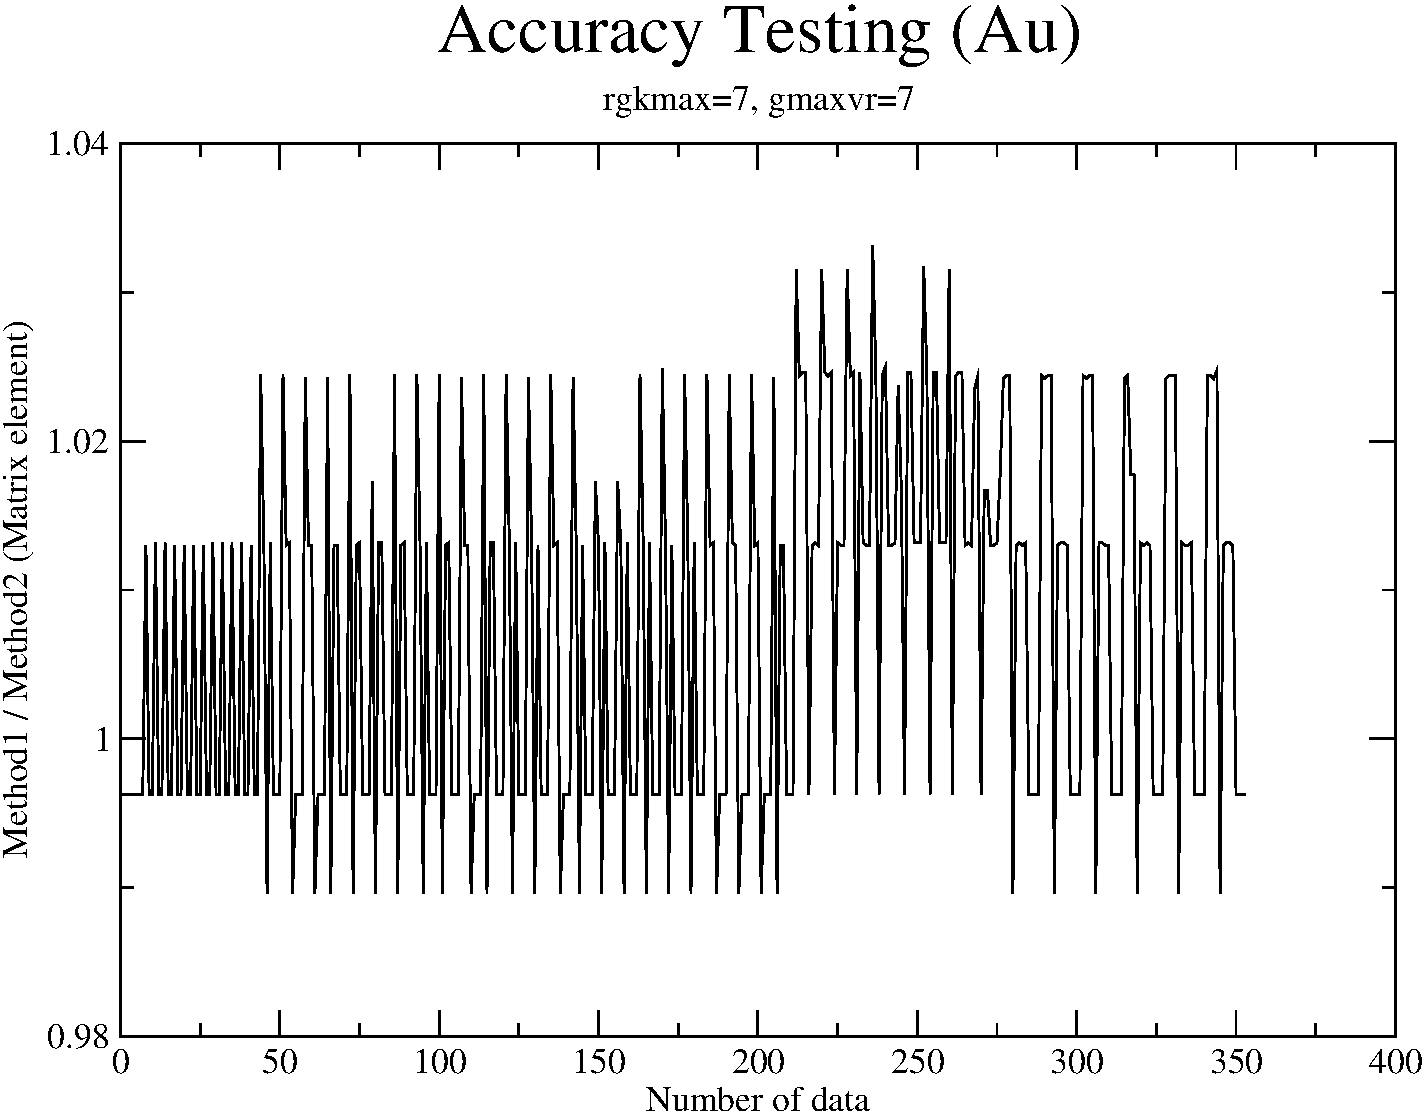
\includegraphics[width=0.5\textwidth]{fort7a7.pdf}
        }%
        \subfigure[rgkmx=5, gmaxvr=12]{%
           \label{fig:second}
           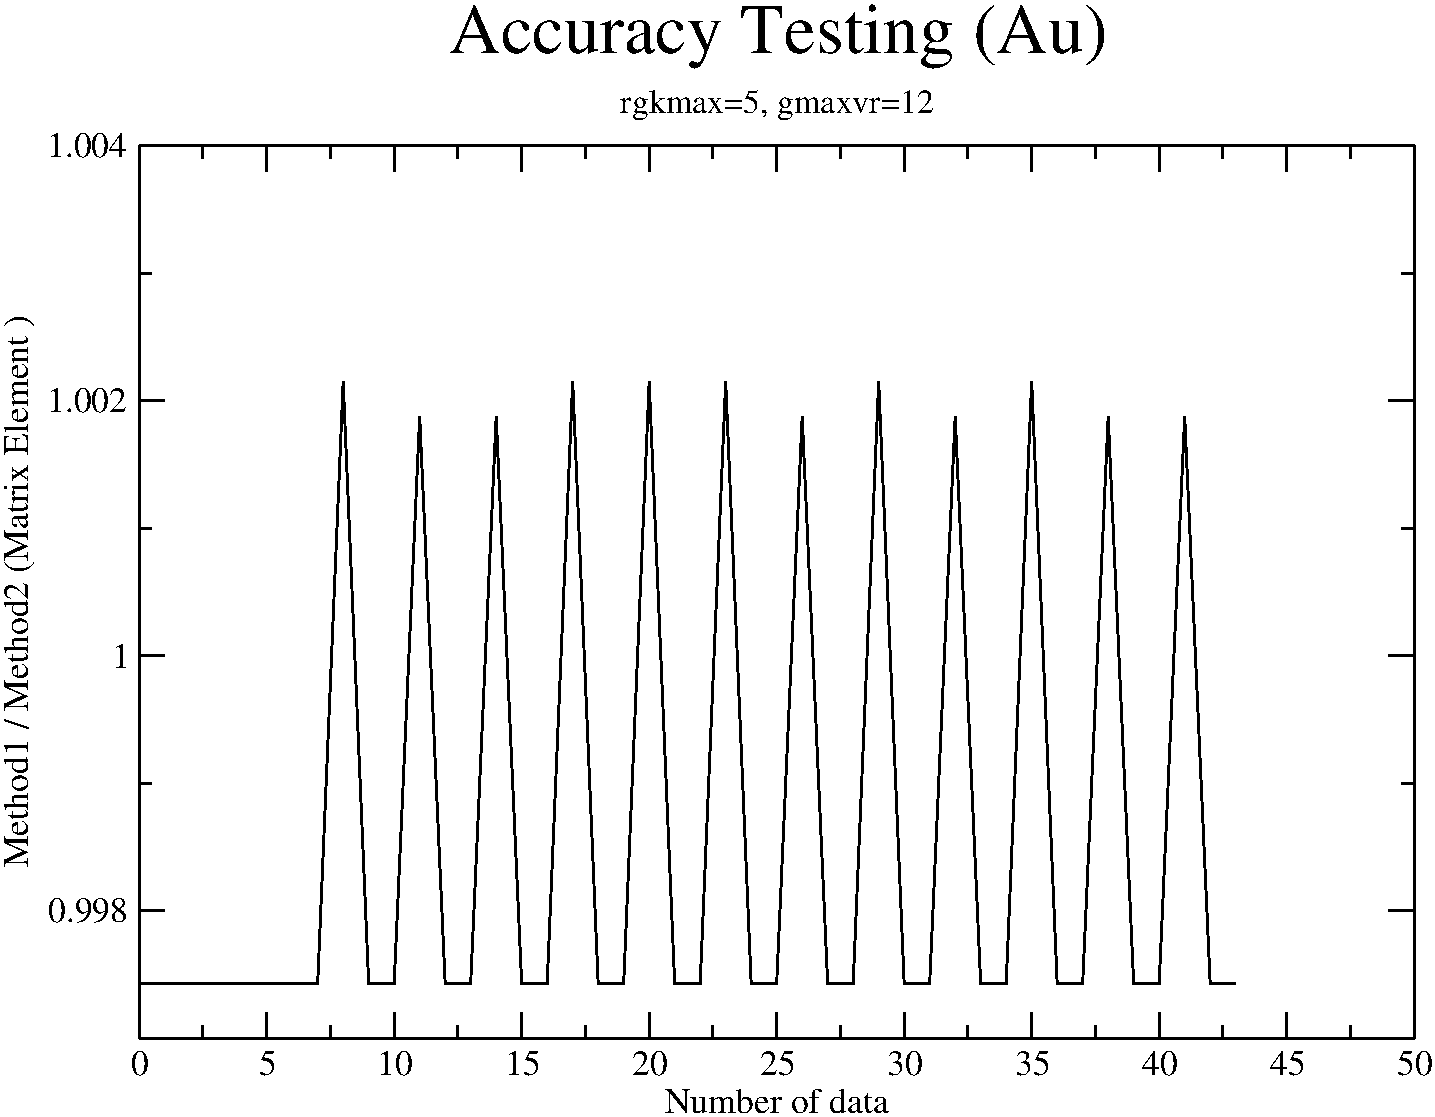
\includegraphics[width=0.5\textwidth]{fort12a5.pdf}
        }\\ %  ------- End of the first row ----------------------%
        \subfigure[rgkmx=7, gmaxvr=12]{%
            \label{fig:third}
            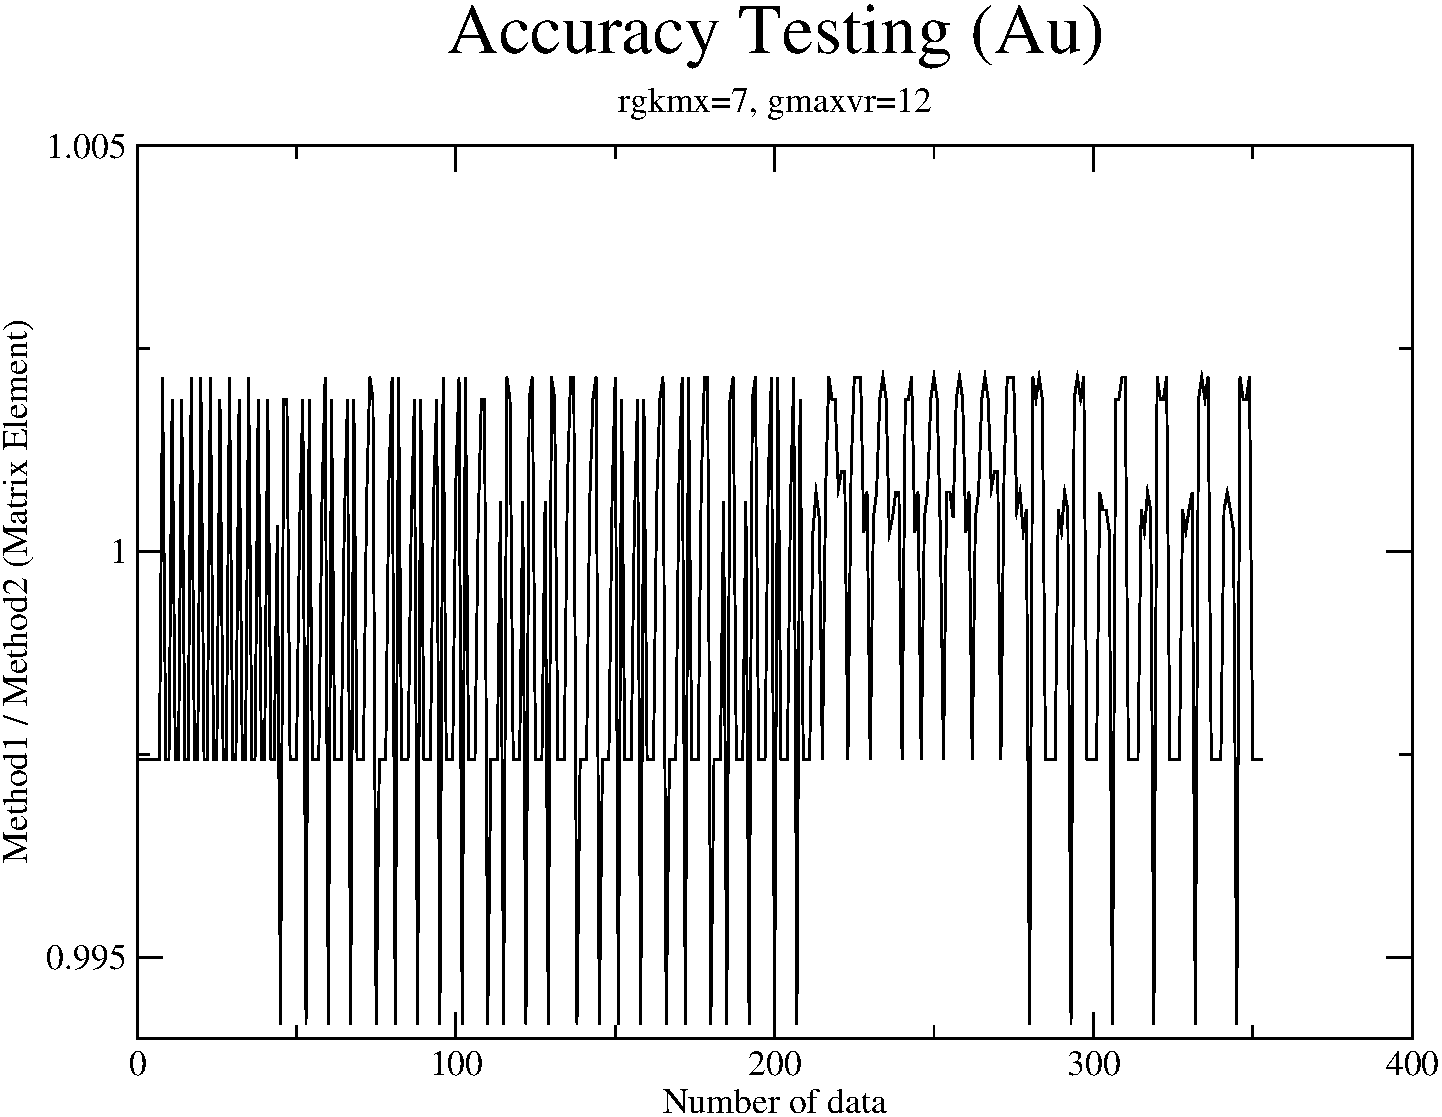
\includegraphics[width=0.5\textwidth]{fort12a7.pdf}
        }%
        \subfigure[rgkmx=7, gmaxvr=12]{%
            \label{fig:fourth}
            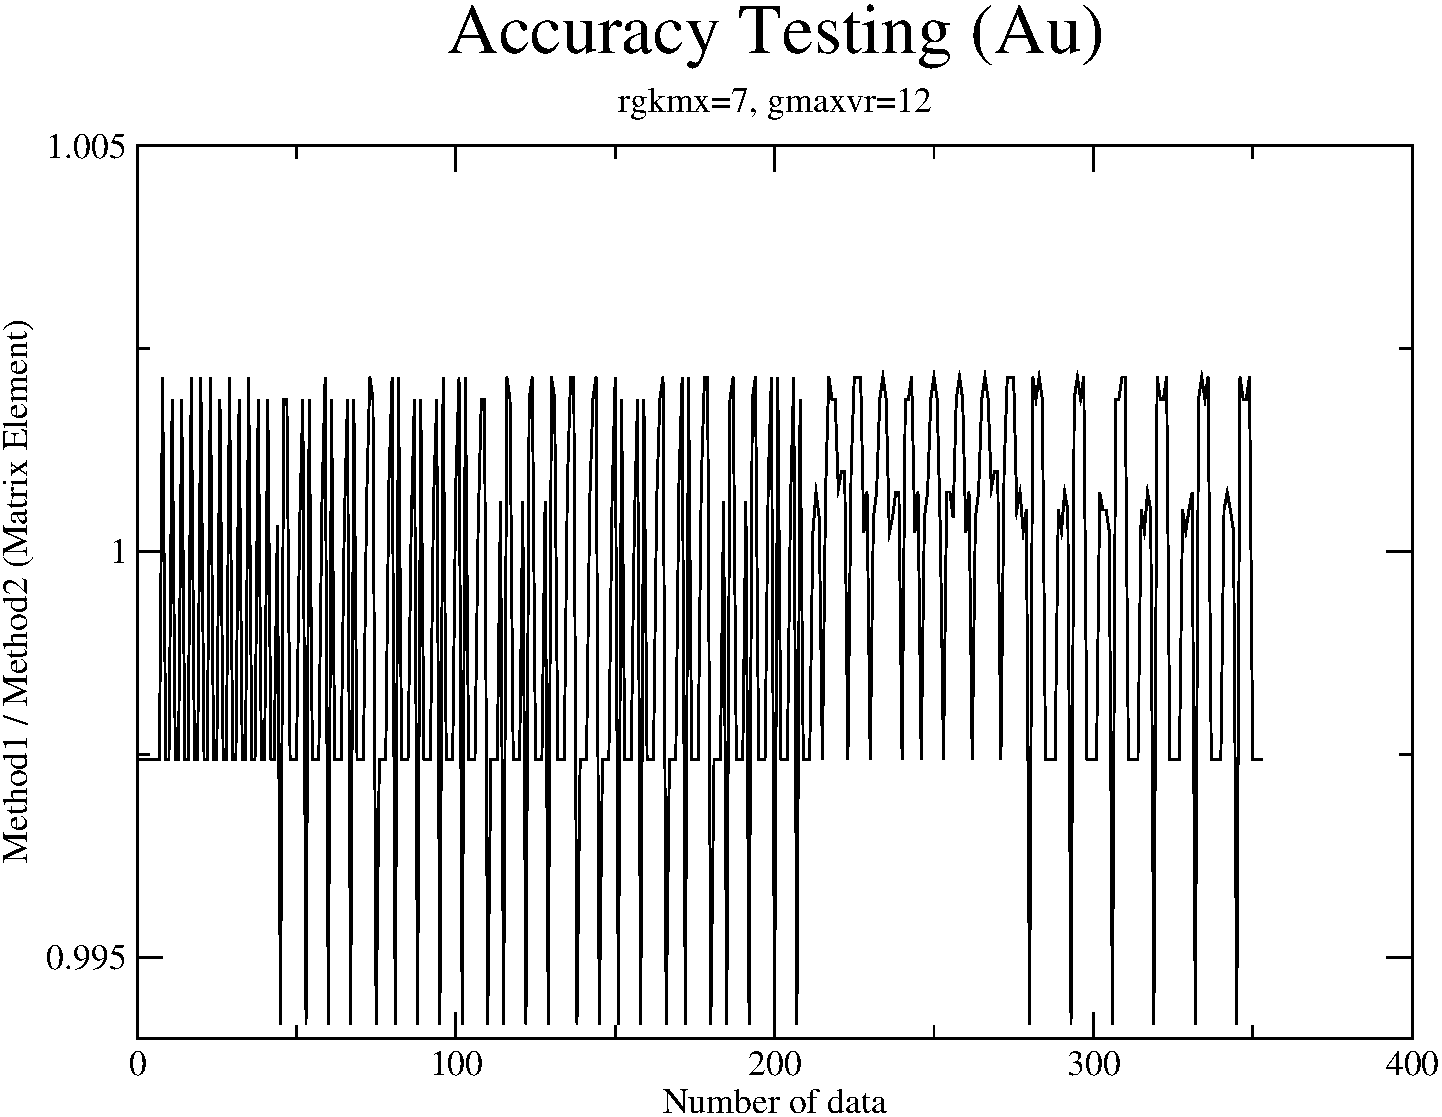
\includegraphics[width=0.5\textwidth]{fort12a7.pdf}
        }\\%
        \subfigure[rgkmx=7, gmaxvr=19]{%
            \label{fig:third}
            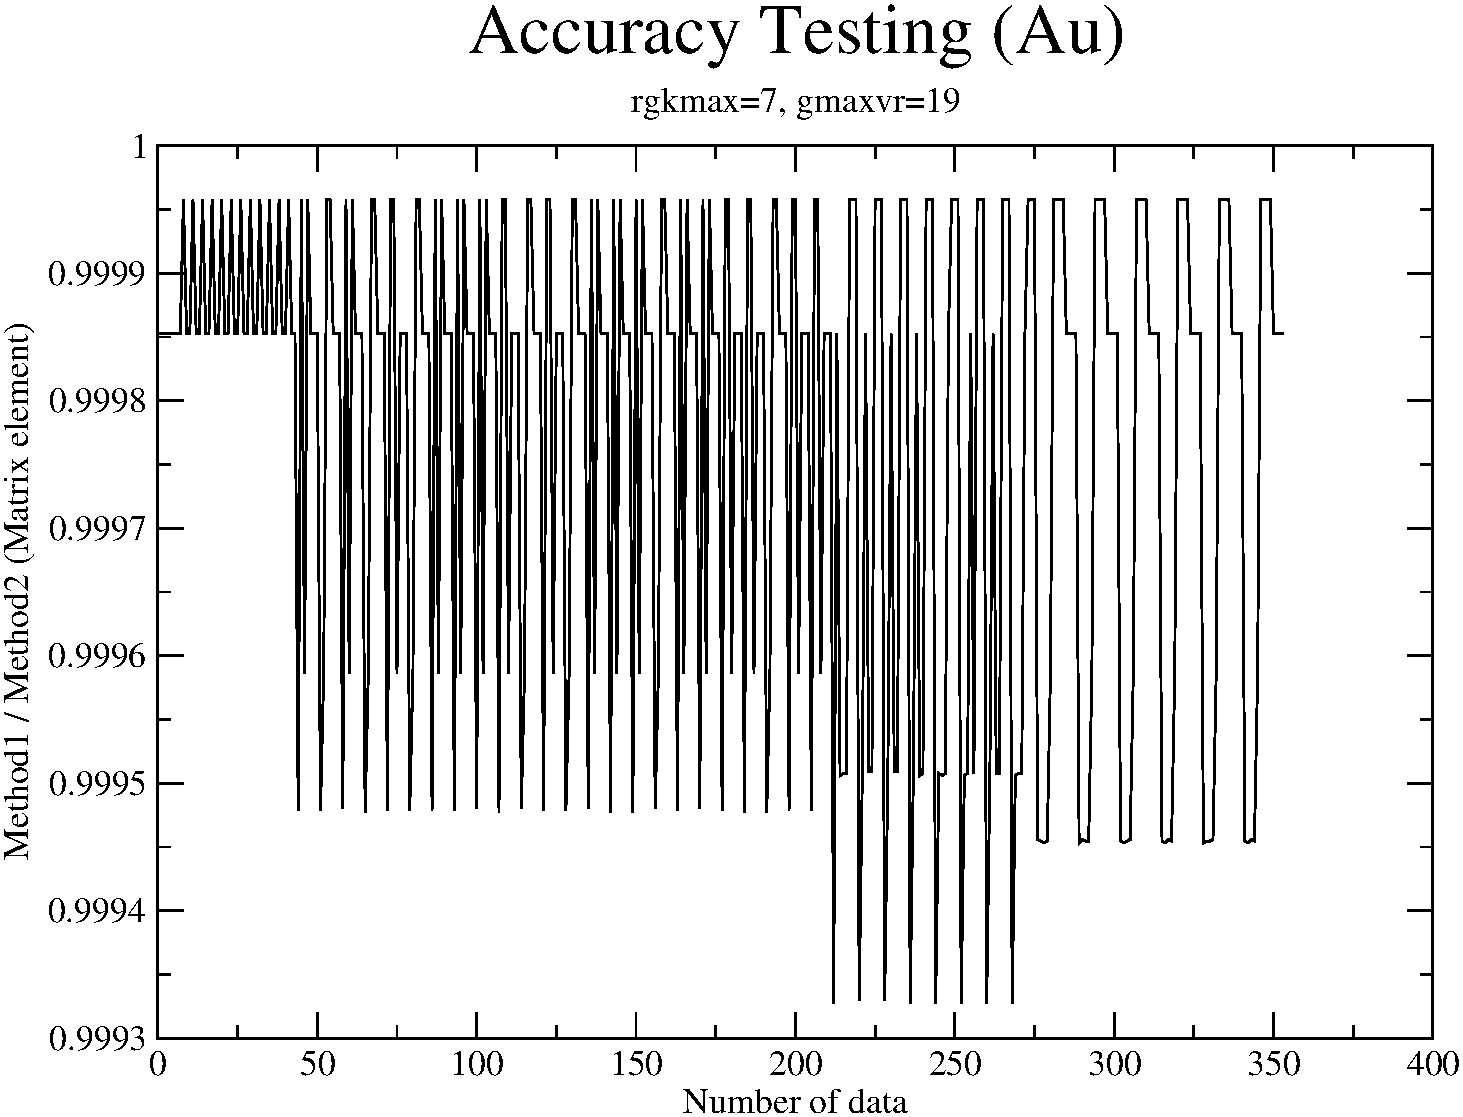
\includegraphics[width=0.5\textwidth]{fort19a7.pdf}
        }%
        \subfigure[rgkmx=9, gmaxvr=12]{%
            \label{fig:fourth}
            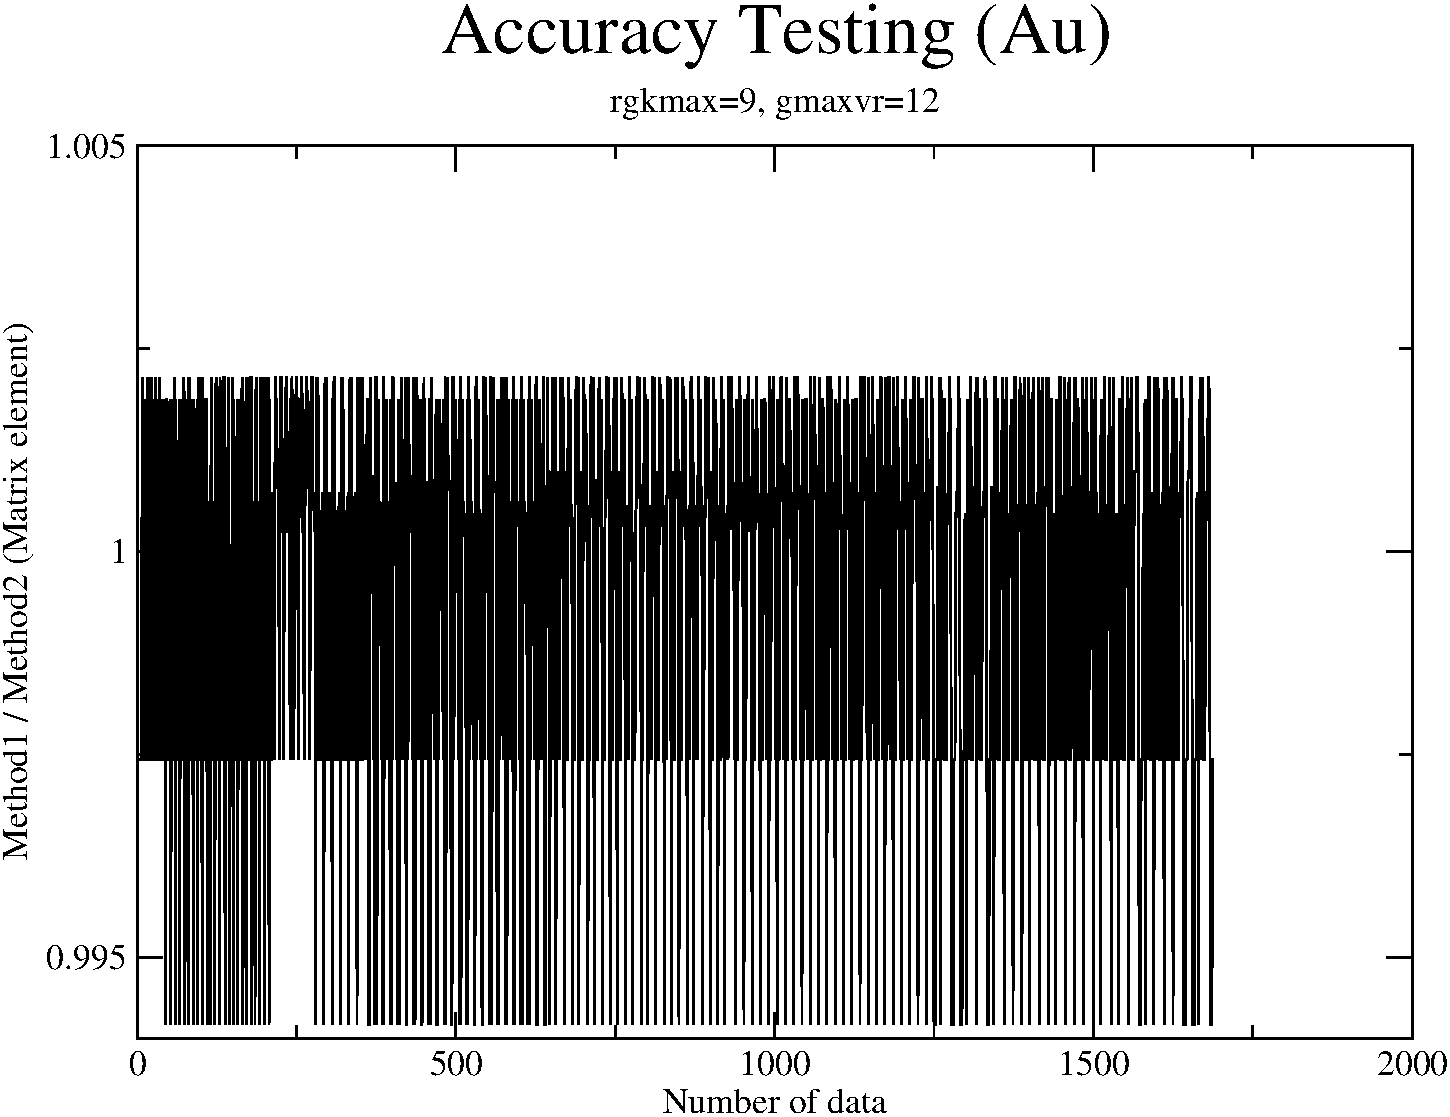
\includegraphics[width=0.5\textwidth]{fort12a9.pdf}
        }%
    \end{center}
    \caption{%
        Accuracy testing for Au, the left column is under the condition fixing the rgkmax value but gmaxvr varys.
        right column is oppsite. Only the matrix element value great than 1E-6 are plotted, and all the imaginary part of value are 
        less than 1E-6, so the imaginary part does not plot in the above figure, for the Y-axis, the Method1 means using equation \ref{sra6}, and Method2 means using 
        equation \ref{sra2}.And the data comes from the first $k$ point during the first self-consistent process.
     }%
   \label{fig:subfigures}
\end{figure}





\vspace{100cm}
From the above figure, first we notice both of them generate the similar result within certain range of difference, so the implementation is correct, then 
we can check how important parameter affect the result. With the default number of $gmaxvr$ and $rgkmax$ by the Exciting code ($gmaxvr$=12, $rgkmax$=7), 
the accuracy is controlled under 0.5\%, here,$gmaxvr$ means maximum length of $G$ for expanding the interstitial density and potential and $rgkmax$ will 
control the number of basis funtion. but when reducing the number $gmaxvr$ to 7,the accuracy is down to 2\% to 3\%.However increasing the number of $rgkmax$, 
the acccuracy is not improve that much, which means the accuracy is quite controlled by the number of $gmaxvr$. Actually, 
we choose the equation \ref{sra6} to implement this SRA affect, because the code will gain more performance than using equation \ref{sra2} under the reasonable number
of $gmaxvr$.
\subsection{Test of matrix element for spin-orbit coupling}

In this section, we first show another derivation of SOC, and then compare the matrix element result like previous section, at last, we will show one concrete example which 
is affected by the SOC.

\begin{equation}\label{soctest1}
\begin{split}
 & H_{j,j'}^{soc} = < \Psi_j(r) | \widehat{H}_{soc}  | \Psi_{j'}(r) >  \\
& =   < \Psi_j(r)  |  \frac{-i}{4 c^2} \boldsymbol{\sigma} [ (\triangledown V(r)) \times \triangledown] |  \Psi_{j'}(r)  > \\
& =  \frac{-i}{4 c^2}   \int_{\Omega} \Psi^{*}_j(r)  \theta_{I}(r)  \boldsymbol{\sigma}  \{ \triangledown V(r) \} \times \{ \triangledown \Psi_{j'}(r) \}  > 
\end{split}
\end{equation}

In the above equation, we can use the Fourier transform for each block of following equaion (like equation \ref{soc2} to \ref{soc3}):
\begin{equation}
  \boldsymbol{\sigma} \theta_{I}(r) \{ \triangledown V(r) \} \times \{ \triangledown \Psi_{j'}(r) \} = f(r) = \sumg<G'> c_{j',k+G'} \expg<(k+G')>
\end{equation}

So if we define $\Psi^{ft}_{j'}(r) = \sumg<G'> c_{j',k+G'} \expg<(k+G')>$ we can write down the equation \ref{soctest1}:

\begin{comment}

\end{comment}

\begin{equation}\label{soctest2}
\begin{split}
& H_{j,j'}^{soc} =   \frac{-i}{4 c^2}   \int_{\Omega} \Psi^{*}_j(r)     \Psi^{ft}_{j'}(r)  >  \\
& = \frac{-i}{4 c^2}   \int_{\Omega} \Psi^{*}_j(r)  \Psi^{fs}_{j'}(r)  \\
& = \frac{-i}{4 c^2}   \sumg<G> c^{*}_{j,k+G} c_{j',k+G} 
\end{split}
\end{equation}

Comparing the above equation \ref{soctest2} with \ref{soc}, we can clear see that the equation \ref{soctest2} is much simplier and better performance, so in the implementaion
we take advantage of the equation \ref{soctest2}, but using \ref{soc} for testing the accuracy even though it is quite time consuming (for each matrix element there are three loops, 
so if each loop in the order of $10^2$, then it is up to the order of $10^{6}$),  so in the implementaion, we use equation \ref{soctest2}.

Now let us examinate these two methods:

\begin{figure}[ht!]
     \begin{center}
        \subfigure[rgkmx=7, gmaxvr=7]{%
            \label{fig:first}
            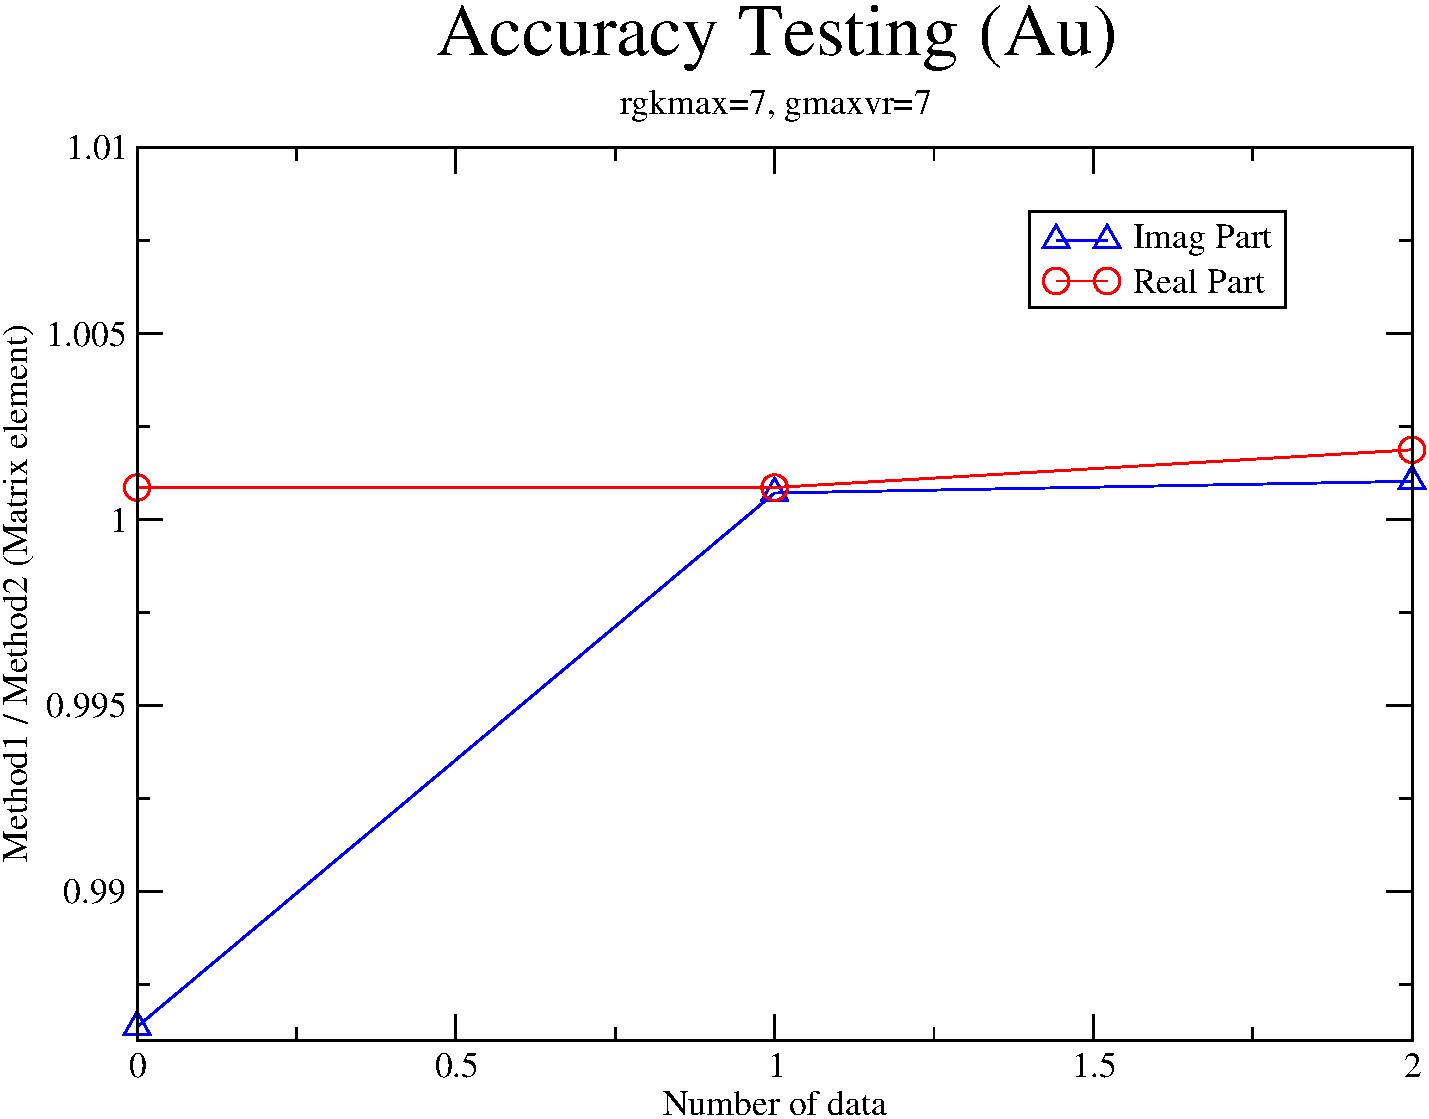
\includegraphics[width=0.5\textwidth]{fort7a7soc.pdf}
        }%
        \subfigure[rgkmx=5, gmaxvr=12]{%
           \label{fig:second}
           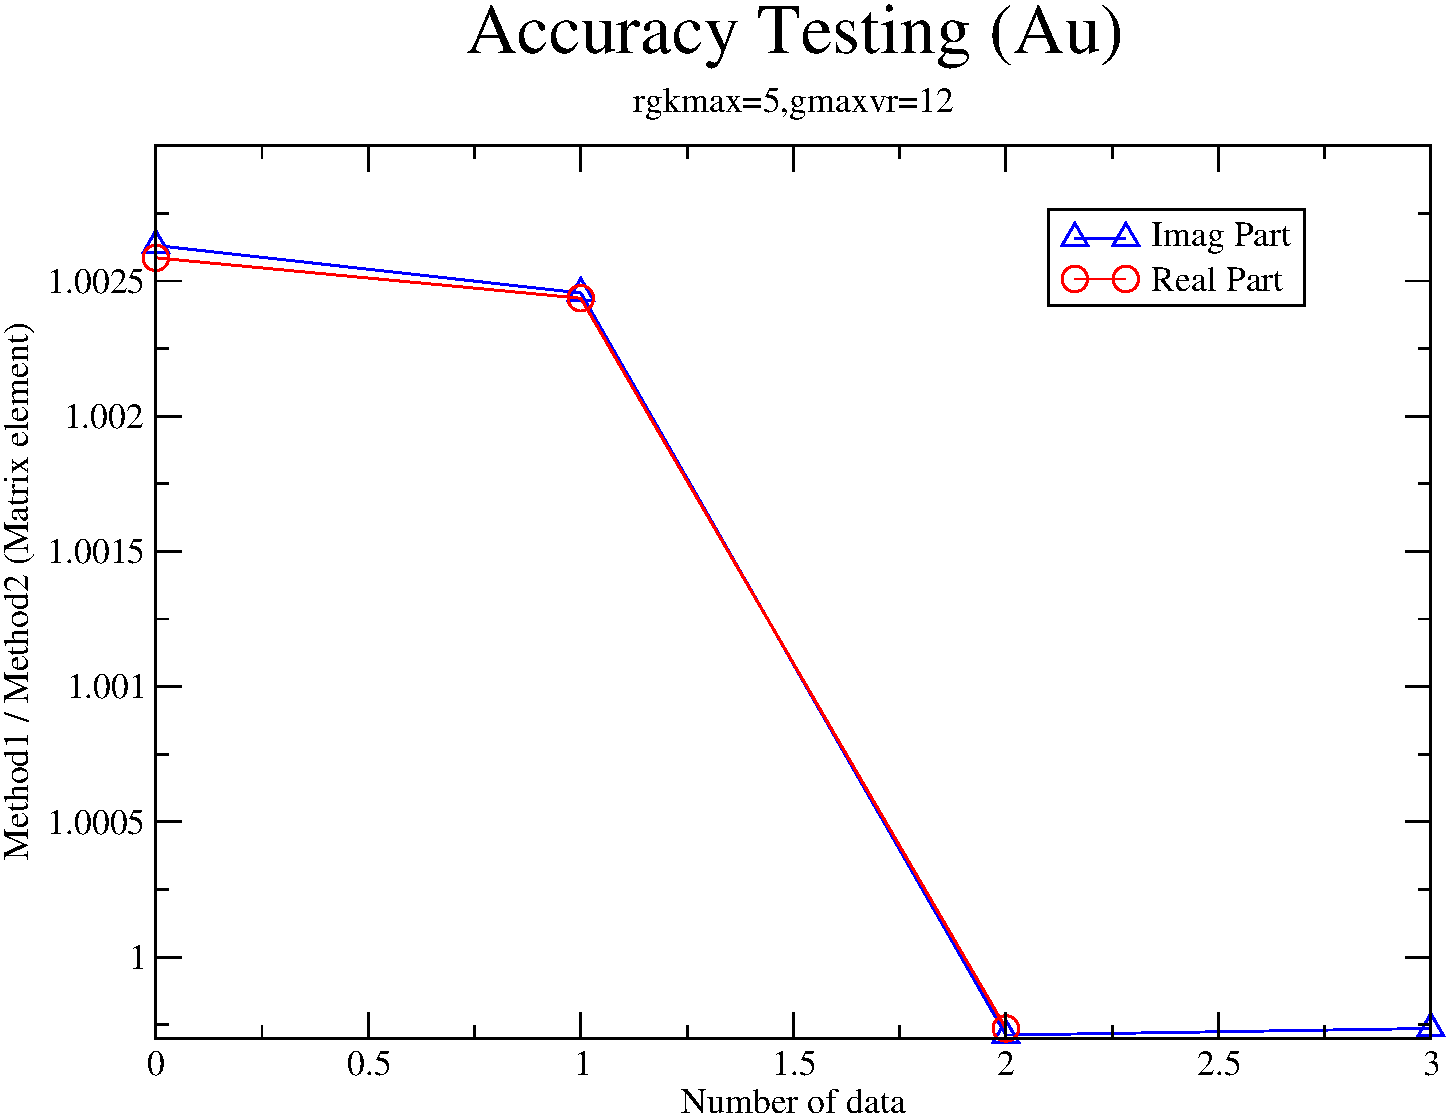
\includegraphics[width=0.5\textwidth]{fort12a5soc.pdf}
        }\\ %  ------- End of the first row ----------------------%
        \subfigure[rgkmx=7, gmaxvr=12]{%
            \label{fig:third}
            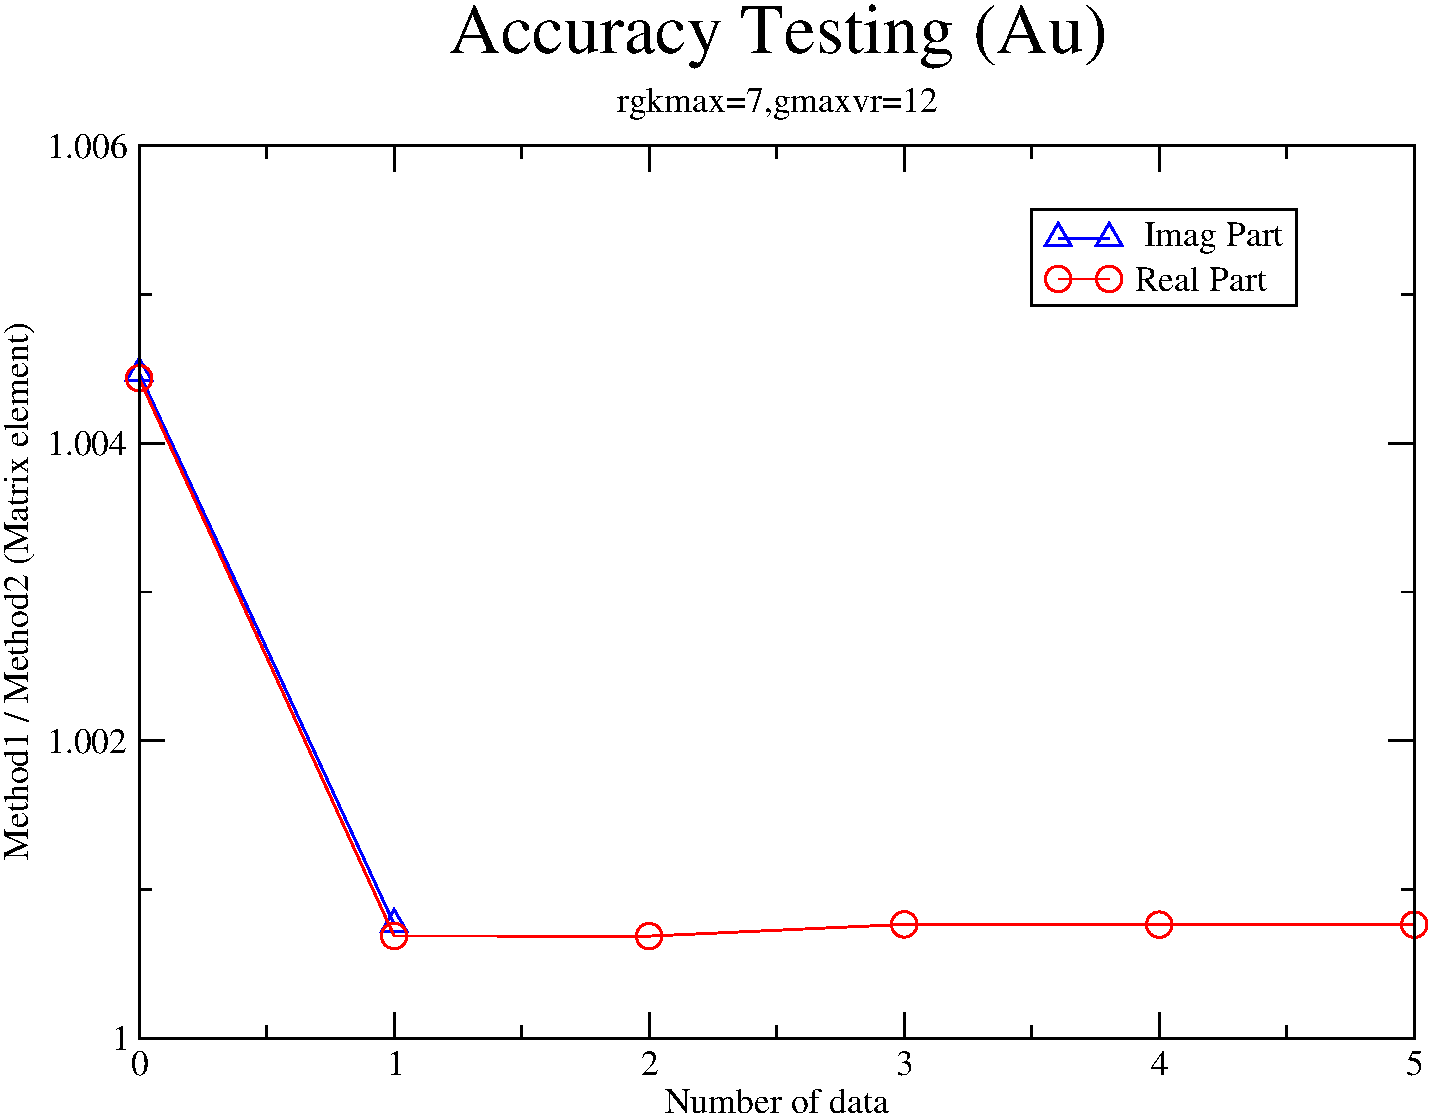
\includegraphics[width=0.5\textwidth]{fort12a7soc.pdf}
        }%
        \subfigure[rgkmx=7, gmaxvr=12]{%
            \label{fig:fourth}
            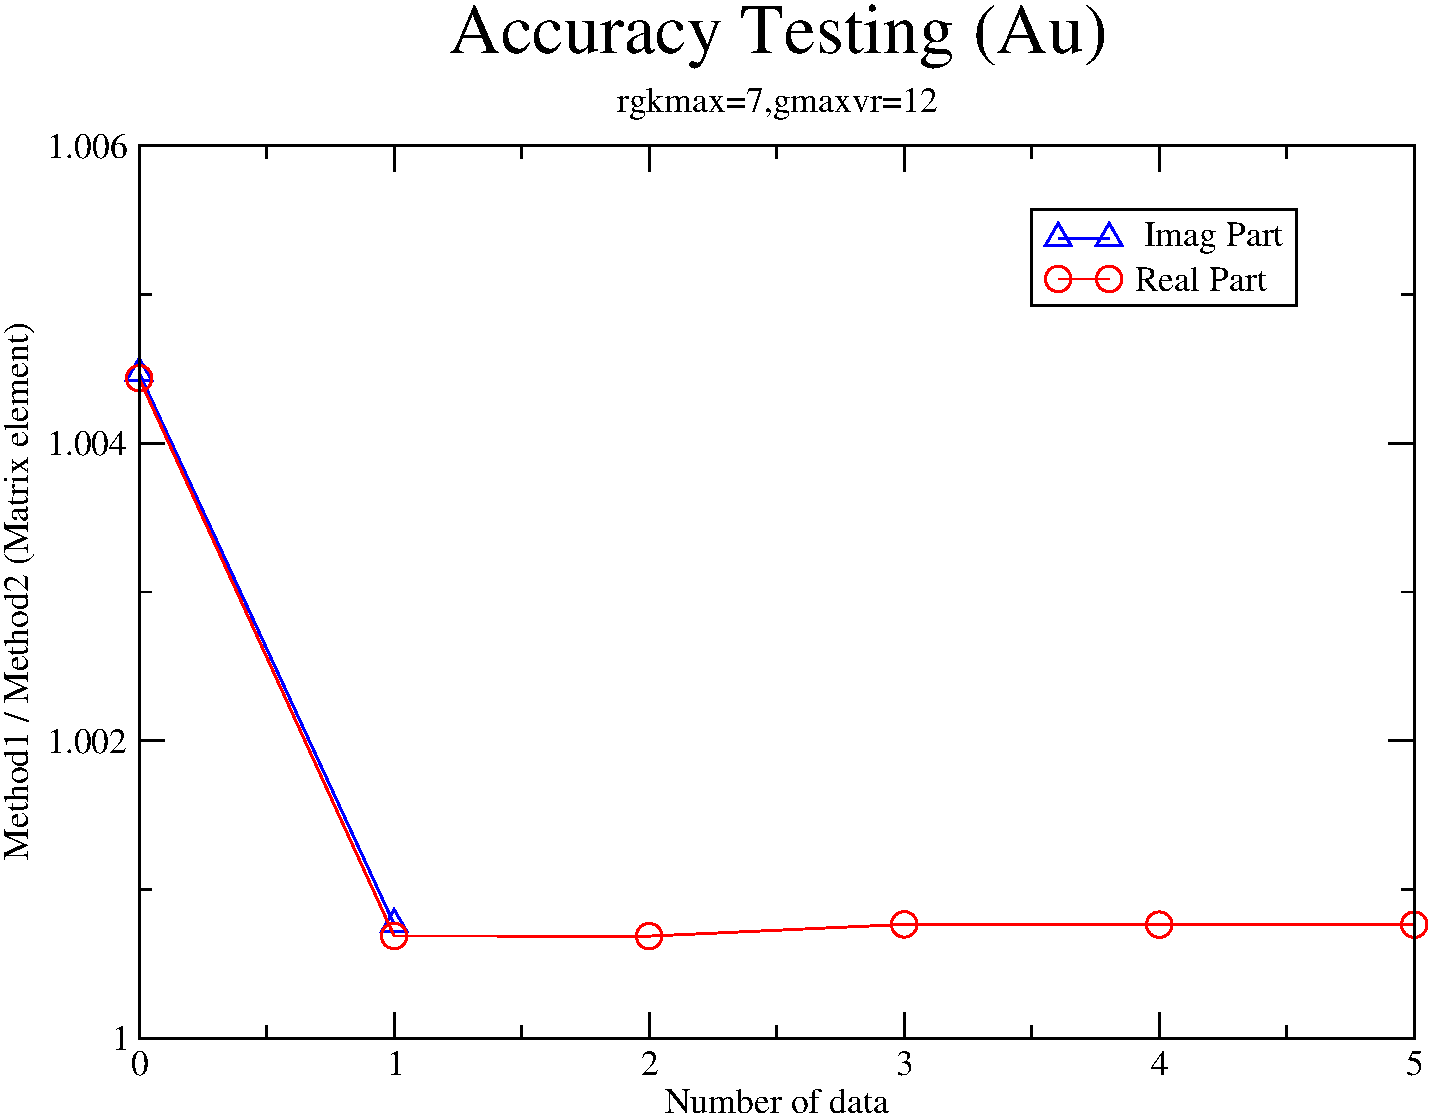
\includegraphics[width=0.5\textwidth]{fort12a7soc.pdf}
        }\\%
        \subfigure[rgkmx=7, gmaxvr=19]{%
            \label{fig:third}
            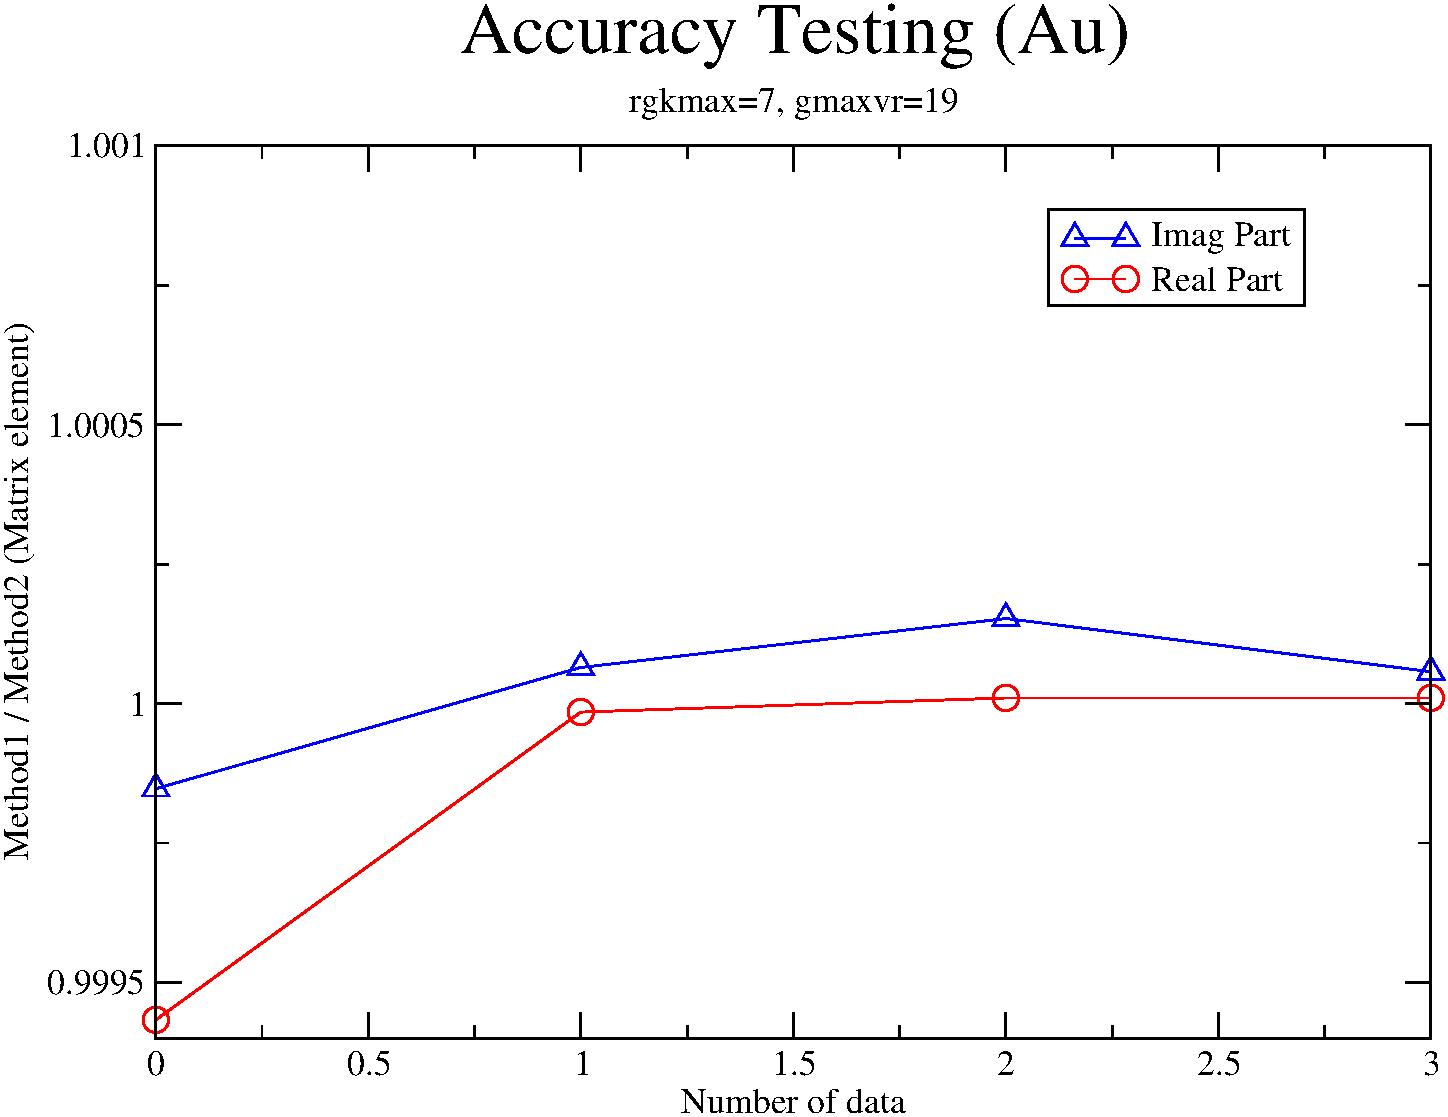
\includegraphics[width=0.5\textwidth]{fort19a7soc.pdf}
        }%
        \subfigure[rgkmx=9, gmaxvr=12]{%
            \label{fig:fourth}
            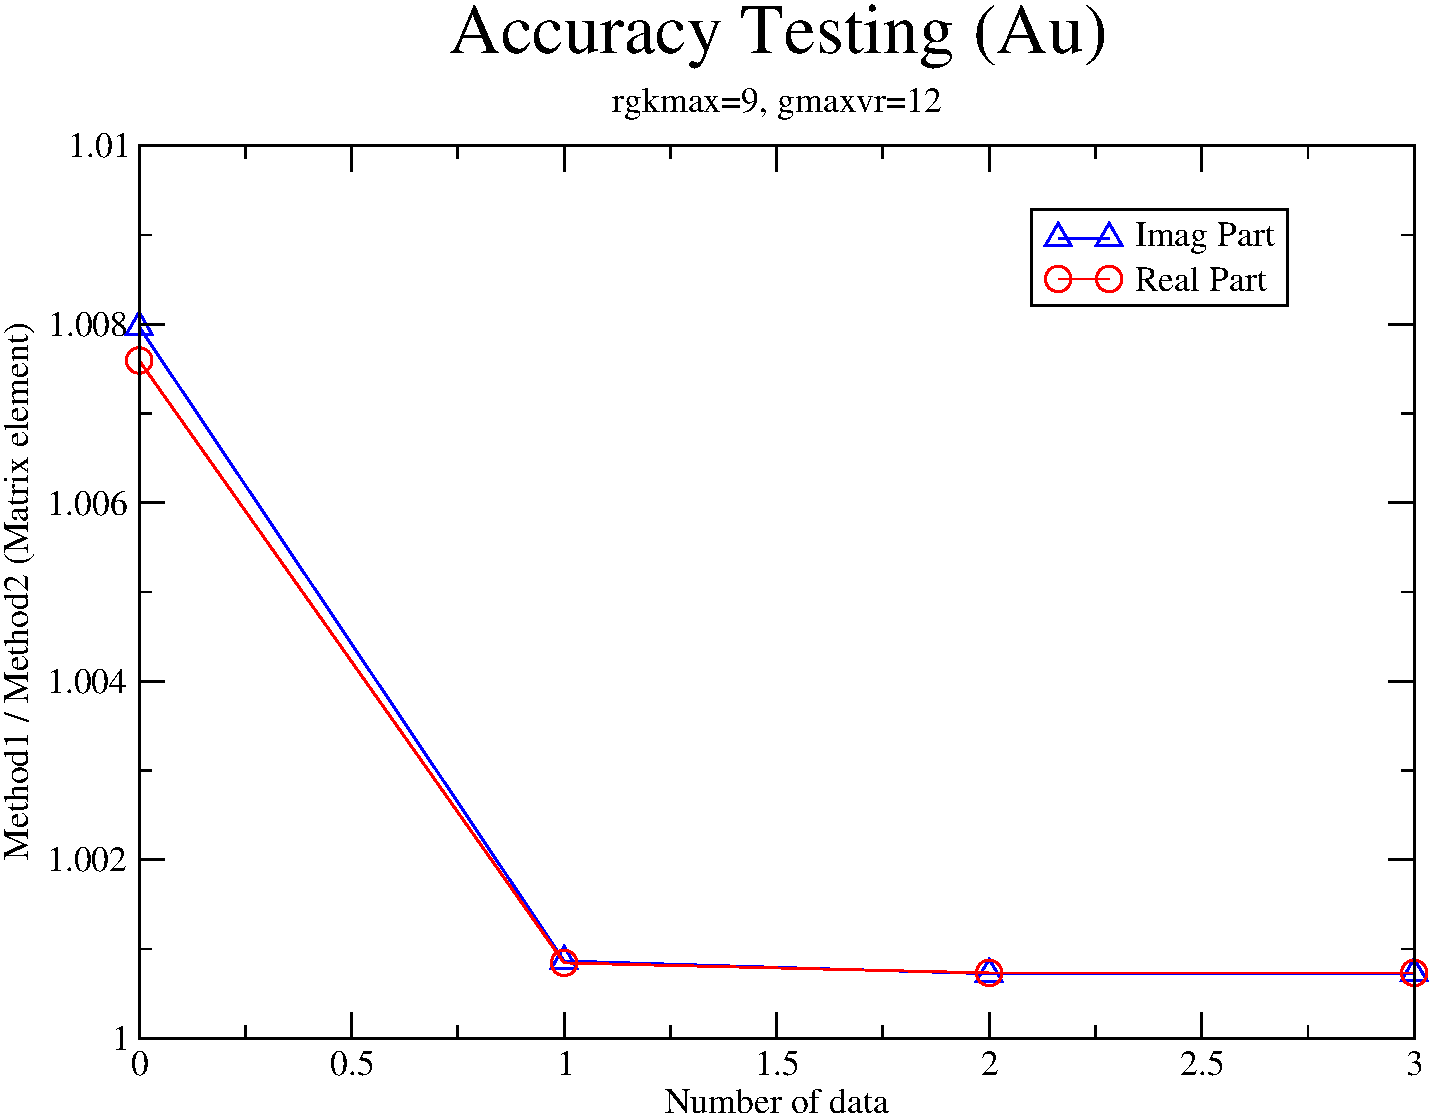
\includegraphics[width=0.5\textwidth]{fort12a9soc.pdf}
        }%
    \end{center}
    \caption{%
        Accuracy testing for Au, the left column is under the condition fixing the rgkmax value but gmaxvr varys.
        right column is oppsite.Only the matrix element value great than 1E-6 are plotted, for the Y-axis, the Method1 means using equation \ref{soctest2},
        and Method2 means using equation \ref{soc}.And the data comes from the first $k$ point during the first self-consistent process.
     }%
   \label{fig:subfigures}
\end{figure}

\vspace{100cm}
From the above figure, we can see both of the methods (equation \ref{soctest2} and \ref{soc}) have the similar result, so the implementation is correct, and then 
it is quite apparently there are less number of data, which means the second variational method is quite efficient. 

We can check that with the default number of $gmaxvr$ and $rgkmax$ by the Exciting code ($gmaxvr$=12, $rgkmax$=7), 
the accuracy is controlled under 0.5\%, but when reducing or incresing the number $gmaxvr$ to 7 or 9, the accuracy is down to 1\% or 0.05\%. However, with the varys of 
$rgkmax$, the accuracy is not change that much.

Let us see the SOC affect on the Dirac point of Graphene, in the case of without spin polarization, there is no splitting energy on the Dirac point, however, in the 
previous researchers' calculation, there are splitting energy on the Dirac point considering the SOC only in the MT, which is in the order of 20 $\mu$Ev,but since 
there is no researchers done the calculation with the SOC contribution on the MT+IR,so I use the implementaion to calculate it, in these calculations, I calculate SOC affect in different radius in MT and MT+IR, then means the SOC in IR as well. 



\begin{figure}[ht!]
\centering
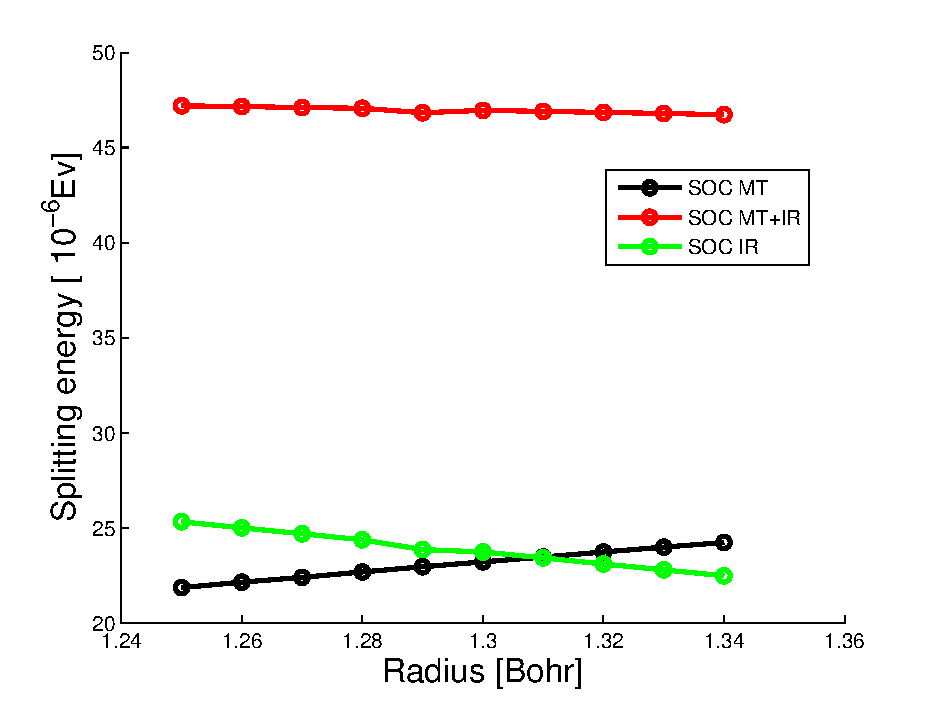
\includegraphics[width=1.0\textwidth]{splittingenergy.pdf}
\caption{Spin-orbit coupling contribution for Graphene}
\end{figure}


From the above figure, we can clear see with the increasing of MT radius, the contribution from SOC in MT increases, but oppsite for SOC in IR, since the whole space is 
contributed by SOC (MT+IR) now, so the total contribute is stable with the varys of MT radius. Also there is one very intriguing phenomenon, the SOC intribution is in the same 
order either in the MT or IR,however, it is believed in the order 20 $\mu$Ev before, but from our calculation,actually it is double since the contribution from IR is ignored from 
all the previous calculation result. 

\chapter{Summary}



\end{document}
